%% TOSEM special section: Human-AI Collaboration in Software Engineering.
%% Journal-first / fast-impact track. Submission deadline 1 September 2026.
%% Formatted per acmart-primary-3 samples/acmsmall-submission.tex.
%%
%% ---------------------------------------------------------------------------
%% ANONYMITY -- ON. The class options below include `anonymous`, so acmart
%% suppresses the author block, affiliations and e-mail addresses on page 1 and
%% in the running heads. To de-anonymise for the camera-ready, drop that one
%% option; nothing else in this file needs changing.
%%
%% What was checked when it was turned on, so a later editor need not redo it:
%%   - acknowledgments thank data-source maintainers, not people or funders
%%   - no repository URL appears anywhere in the paper
%%   - the earlier version of this work is referred to but never cited, so the
%%     bibliography carries no self-identifying entry
%%   - no funding statement
%% Verified on the built PDF three ways, because extracted text alone misses the
%% usual failure: no name, e-mail or affiliation in the text; no /Author
%% metadata key; and no match in a raw string scan of the PDF stream.
%%
%% The body refers to "the conference version" where it reports what that
%% version claimed and how this one corrects it. That phrasing names no venue
%% and no author, and the comparison is the paper's argument rather than
%% incidental, so it stays. Journal-first eligibility is declared on the
%% submission form, not in the manuscript.
%% ---------------------------------------------------------------------------
\documentclass[acmsmall,review,anonymous,screen]{acmart}

%% acmart already loads booktabs, graphicx, pifont and hyperref; re-loading them
%% risks an option clash and counts as modifying the template.
\usepackage{amsmath}
\usepackage{array}
\newcolumntype{R}[1]{>{\raggedright\arraybackslash}p{#1}}
\usepackage{tikz}
\usepackage{pifont}   %% acmart's own pifont load is conditional; \ding needs this

\emergencystretch=3em

\setcopyright{acmlicensed}
\acmJournal{TOSEM}
\acmYear{2027}
\acmVolume{0}
\acmNumber{0}
\acmArticle{0}
\acmMonth{8}
\copyrightyear{2027}
\acmDOI{}

\received{1 September 2026}

\title[When Query Rewriting Loses the Documents]{When Query Rewriting Loses the
Documents: An Adaptive Multi-Agent RAG Architecture for Software Ecosystem
Update Monitoring}

\author{Shradha Devendra Pujari}
%% TODO before camera-ready: add the author's real ORCID.
%% \orcid{0000-0000-0000-0000}
\affiliation{%
  \institution{University of the Pacific}
  \department{Department of Computer Science}
  \city{Stockton}
  \state{CA}
  \country{USA}}
\email{s_pujari@u.pacific.edu}

\author{Solomon Berhe}
%% TODO before camera-ready: add the author's real ORCID.
%% \orcid{0000-0000-0000-0000}
\affiliation{%
  \institution{University of the Pacific}
  \department{Department of Computer Science}
  \city{Stockton}
  \state{CA}
  \country{USA}}
\email{sberhe@pacific.edu}

\begin{document}

\begin{abstract}
Software ecosystems produce release notes, security advisories, version control
records, and community discussions, and answering a question about a software
update usually requires combining several of them. Retrieval-Augmented
Generation (RAG) is a natural fit, and a common design pattern decomposes the
pipeline into specialized agents, with a query-rewriting agent normalizing user
terminology to the vocabulary of technical documents.

This paper reports two evaluation defects, each of which made that pattern
look decisively better or decisively worse than a single-agent baseline, and
what the comparison looks like once both are removed. We built an adaptive
multi-agent RAG architecture for software update questions --- specialized
agents for query rewriting, retrieval, evaluation, and orchestration, with a
retrieval-level feedback loop and a persistent term-weight memory --- and
measured a 17.2\% retrieval improvement over a single-agent baseline on a
keyword-overlap quality score of our own design. Re-scored with standard
information-retrieval metrics over pooled relevance judgments, the same system
\emph{lost} to the same baseline (nDCG@3 0.145 versus 0.765; paired deficit
0.620, exact Wilcoxon $p=0.016$, $n=10$). We traced the deficit to a wiring
fault --- the rewritten query \emph{replaced} the user's wording at every
retrieval endpoint, so documents matching the user's own phrasing were never
fetched --- and repaired it by issuing both phrasings and unioning the pools,
which brought the pipeline to parity. Then a 500-question run scored 0.34 lower
than a 300-question run on the same questions with nothing changed, and the
second defect surfaced: the benchmark's questions are the titles of real
community posts, the live corpus returns the post a title came from, and the
judge marks it relevant. The question's own source post sat in 72--98\% of the
top-$k$ lists behind every retrieval number we had reported, and it was
precisely the document the rewrite had been losing. Struck from the candidate
pool at fetch time and re-measured on 500 questions across 24 ecosystems, every
arm --- multi-agent, single-agent, and rewrite-only --- retrieves at nDCG@3
0.30--0.31, with no paired difference exceeding 0.015.

We draw four conclusions for practitioners building agentic software
engineering tools. First, a benchmark mined from the same live sources a system retrieves from
leaks its own answer key, and the leak is invisible to paired comparison because
every arm draws on it equally; it shows only in absolute levels, and we found it
only because a level moved between two runs that should have agreed. Second, a
bespoke retrieval-quality metric can invert the ordering that standard IR
metrics produce, and standard IR metrics computed over a leaking corpus can
manufacture a five-fold deficit out of a fetch fault that, leak-free, costs
nothing measurable --- so architectural claims resting on either are not safe
without the candidate pool exposed and counted. Third, an apparent 0.23 faithfulness deficit for the
multi-agent system proved to be an artifact of answer \emph{format} --- a
structured template judged against fluent prose --- and vanished when the same
retrieval was synthesized through the baseline's own prompt (0.919 versus
0.929). Fourth, and least comfortable: with both defects repaired and the
synthesis model held constant, the multi-agent pipeline \emph{matches} rather
than beats the single-agent baseline on retrieval (nDCG@3 0.304 versus 0.301,
$n=500$, leak-free) at roughly twice the latency, so decomposition per se is not
what produced the original result. We release the architecture, the evaluation
harness with the leak excluded by construction, and a 500-question benchmark
mined from live release, advisory, and community sources; these are available to reviewers on request and will be
published on acceptance.
\end{abstract}

\begin{CCSXML}
<ccs2012>
   <concept>
       <concept_id>10002951.10003317.10003338</concept_id>
       <concept_desc>Information systems~Retrieval models and ranking</concept_desc>
       <concept_significance>500</concept_significance>
       </concept>
   <concept>
       <concept_id>10002951.10003317.10003359</concept_id>
       <concept_desc>Information systems~Evaluation of retrieval results</concept_desc>
       <concept_significance>500</concept_significance>
       </concept>
   <concept>
       <concept_id>10011007.10011074.10011081</concept_id>
       <concept_desc>Software and its engineering~Software maintenance tools</concept_desc>
       <concept_significance>300</concept_significance>
       </concept>
   <concept>
       <concept_id>10010147.10010178.10010179</concept_id>
       <concept_desc>Computing methodologies~Natural language processing</concept_desc>
       <concept_significance>300</concept_significance>
       </concept>
 </ccs2012>
\end{CCSXML}

\ccsdesc[500]{Information systems~Retrieval models and ranking}
\ccsdesc[500]{Information systems~Evaluation of retrieval results}
\ccsdesc[300]{Software and its engineering~Software maintenance tools}
\ccsdesc[300]{Computing methodologies~Natural language processing}

\keywords{Multi-Agent Systems, Retrieval-Augmented Generation, Query Rewriting,
Retrieval Evaluation, Software Ecosystem Monitoring, Negative Results,
Self-Improving Agents, RLAIF}

\maketitle

\section{Introduction}

Modern software ecosystems produce a diverse collection of documents, including release notes, security advisories, version control records, and online community discussions. These documents contain information about software updates, vulnerabilities, compatibility issues, and deployment considerations. Answering software update--related questions often requires integrating information from multiple sources.

Each of these artefacts has been studied in its own right. Release notes are known to be produced inconsistently and to omit information their readers need, which has motivated work on summarising and generating them automatically~\cite{abebe2016releasenotes,moreno2017arena,bi2022releasenotes} and on the discipline of version identifiers themselves~\cite{guo2025verlog}. Developers routinely turn to community platforms and web search when documentation is insufficient~\cite{xia2017websearch,zhang2018apimisuse}, and the reliability of what they find there is an active question~\cite{kabir2024stackoverflow,stolee2025codesearch}. The task studied here sits across these sources rather than within any one of them.

Software update information is frequently accessed through natural language questions. Developers, system administrators, and users commonly ask colleagues about software updates or seek information through online community platforms. Answering such questions often requires locating relevant documents, reviewing information from multiple sources, and evaluating the consistency of available documents. Systems that generate accurate source-grounded answers can reduce the effort required to retrieve, read, and synthesize information from software ecosystem documents.

Retrieval-Augmented Generation (RAG) systems have emerged as a promising approach for answering such questions by combining document retrieval with large language models to generate answers grounded in external information~\cite{lewis2020rag}. Conventional single-agent RAG systems typically perform query understanding, retrieval, evaluation, and answer generation within a single reasoning process. This can result in vocabulary mismatch between user questions and retrieved documents~\cite{gao2024dmqr}, limited handling of domain-specific terminology, and the absence of feedback mechanisms for correcting retrieval errors \cite{cook2025rag}.

Recent multi-agent RAG systems decompose retrieval and reasoning into multiple specialized agents~\cite{wang2024mainrag, nguyen2025marag}. Most existing evaluations focus on general question-answering benchmarks, whereas software update questions require combining information from heterogeneous software ecosystem documents. In addition, the role of feedback-based adaptation in multi-agent RAG systems for software update question answering has received limited empirical evaluation~\cite{ma2023rafe}.

This paper presents an Adaptive Multi-Agent RAG Architecture for answering software update questions \cite{he2025,joshi2025review}. The architecture consists of specialized agents for query rewriting, retrieval, evaluation, and orchestration connected through a feedback loop \cite{adimulam2026,roman2026}.

\subsection{A Result We Did Not Expect}

Our first evaluation followed what is, judging by the literature, common
practice: we defined a retrieval-quality score for the domain --- keyword and
source overlap between the question and the retrieved set --- and compared the
multi-agent architecture against a single-agent baseline on 50 real user
questions. The architecture improved that score by 17.2\% ($t(49)=2.32$,
$p=0.020$), improving in every question category. That is the result reported in
the conference version of this work.

Re-scoring the same pipeline with standard information-retrieval metrics ---
nDCG@$k$, Recall@$k$, and MRR over relevance judgments pooled across systems ---
reversed the ordering. The single-agent baseline reached nDCG@3 of 0.765; the
multi-agent architecture reached 0.145, a paired per-query deficit of 0.620
(bootstrap 95\% CI $[0.348, 0.865]$, exact Wilcoxon signed-rank $p=0.016$,
$n=10$). A 17.2\% advantage on one metric
coexisted with a factor-of-five deficit on another, over the same questions, the
same corpus, and the same retrieved documents.

Metric disagreements of this size usually indicate that one metric is measuring
something other than what it claims. That was true here twice over, and neither
time in the direction we assumed. Investigating the gap produced the diagnosis
the first version of this paper was built around:

\begin{quote}
\emph{The query-rewriting agent's output replaced the user's wording at every
retrieval endpoint. Of the 23 relevant documents the single-agent baseline
retrieved across the evaluation set, 22 were never fetched by the multi-agent
pipeline at all.}
\end{quote}

The rewritten query was not retrieving the wrong documents from a correct
candidate set --- a ranking problem, which is how we first read the evidence and
how the vocabulary-mismatch framing in the literature invites one to read it.
It was constructing a different, smaller candidate set from which the answer was
largely absent.

That diagnosis was correct as far as it went, and the remedy it implied ---
issue both phrasings, union the pools --- brought the multi-agent pipeline to
parity with the baseline on every sample we drew, at $n=10$, $n=100$, and
$n=300$. It was also, we later learned, measuring the wrong thing. The 23
``relevant documents'' were, overwhelmingly, the questions' own source posts.

The benchmark's questions are the titles of real community posts, chosen for
that reason: they are the questions people actually asked. The system retrieves
from the same live community feed those posts were drawn from. So the feed
returns the post a title came from, the relevance judge --- correctly, by its
instructions --- marks a document that \emph{is} the question as relevant to
it, and every retrieval metric rewards the arm that found it. The single-agent
baseline, issuing the title verbatim, found it on 7 of the 10 diagnostic
questions; the multi-agent pipeline, issuing a paraphrase, found it on none.
That is the five-fold deficit. The union fetch restored the verbatim phrasing,
the own post came back, and nDCG@3 rose from 0.188 to 0.765 --- with the own
post in all ten top-3 lists. Struck from the candidate pool, the same runs read
0.309 before the ``repair'' and 0.216 after it.

We did not find this by inspection. We found it because a 500-question run
scored 0.34 lower than a 300-question run on the same 300 questions, with the
code, judge, and reranker unchanged: the live feed had aged past most of the
source posts in the two weeks between them, and the leak, which had inflated
every arm equally and so never appeared in a paired comparison, appeared as a
drop in the absolute level. Re-measured with the own post excluded at fetch time
(Section~\ref{sec:leak}), every arm --- the full pipeline, the baseline, and a
rewrite-only arm with no union fetch at all --- retrieves at nDCG@3 0.30--0.31
on 500 questions, and no paired difference exceeds 0.015.

That substitution harms retrieval is not a new result, and we want to be exact
about what is ours. It is documented in the query-rewriting literature this
paper itself cites: query2doc reports that retrieving with the generated text
alone scores below not rewriting at all and recovers the loss by concatenating
the original query~\cite{wang2023query2doc}, DMQR-RAG retrieves with the original
alongside its rewrites and merges the results~\cite{gao2024dmqr}, and both the
fuse-the-result-lists remedy and the argument that re-ranking cannot recover what
a query never retrieved were published in 2008~\cite{zighelnic2008drift}. The
contribution here is not that finding, nor the remedy, and it is no longer the
fetch-loss diagnosis either, since the documents the fetch lost turned out to be
the questions themselves. It is the pair of evaluation defects and the order in
which they hid each other: a bespoke metric that rewarded the rewriter's
vocabulary made the architecture look better than the baseline; a benchmark
that leaked its own questions into the corpus made the architecture look five
times worse; and the second defect was invisible to exactly the paired,
pooled-judgment methodology we adopted to escape the first, because it inflated
every arm by the same amount. We report the procedure that found each --- expose
the candidate pool and count documents rather than read scores; re-run identical
questions at an interval and treat a moving absolute level as a finding --- and
the leak-free measurement that results.

\subsection{Contributions}

\begin{itemize}
  \item \textbf{A benchmark--corpus leak specific to live-source RAG, and its
  measurement.} A benchmark whose questions are mined from the sources the
  system retrieves from returns the question's own source document as a
  relevant hit. In every retrieval table we had reported, at $n=10$, 100, and
  300, the question's own post occupied 72--98\% of top-$k$ lists and was the
  only judged-relevant document for a third to a half of the questions. Because
  every arm retrieved it at the same rate, paired comparisons never showed it;
  a drop in absolute level between two runs on identical questions did. We give
  the mechanism, a post-hoc correction that strikes the document from ranking
  and judgments, a fetch-time exclusion that removes it by construction, and a
  leak-free measurement on 500 questions (Section~\ref{sec:leak}).

  \item \textbf{A reading of query-rewriting drift that the leak reverses.}
  Substituting a rewritten query for the user's own is known to hurt
  retrieval~\cite{wang2023query2doc,gao2024dmqr,zighelnic2008drift}, and we
  observed the textbook signature: 22 of 23 relevant documents never fetched,
  MRR rising under three successively stronger rerankers while nDCG@$k$ stayed
  flat. What the rewrite lost, on this benchmark, was the document that matched
  the user's wording \emph{because it was the user's wording} --- the source
  post. Leak-free, a rewrite-only arm with no union fetch retrieves within 0.006
  nDCG@3 of the verbatim baseline (Section~\ref{sec:leak}). We report the
  diagnostic because it worked --- it located the lost documents --- and the
  reversal because the documents it located were not answers.

  \item \textbf{Evidence that a domain-specific retrieval metric can invert the
  conclusion.} The same architecture, questions, and documents yield opposite
  orderings under our keyword-overlap score and under pooled-judgment IR
  metrics. We report both, with the pooling protocol and judge configuration, as
  a caution for agentic-system evaluations that define their own quality scores
  --- and we report that the pooled-judgment metrics, computed over a leaking
  corpus, were themselves measuring a lookup rate.

  \item \textbf{An honest accounting of what multi-agent decomposition bought.}
  Leak-free, on 500 questions, the multi-agent pipeline retrieves at nDCG@3
  0.304 against the baseline's 0.301, with 418 of 500 questions tied and no
  metric differing by more than 0.015, at approximately twice the latency. The
  parity held in every leaking sample as well; it is the one result the leak did
  not touch. We report it rather than the improvement the original metric
  showed, and discuss what would constitute evidence for decomposition in this
  domain.

  \item \textbf{An architecture and adaptation mechanism for software ecosystem
  monitoring.} Vendor-aware retrieval across release notes, security advisories,
  and community discussions, a deterministic evaluator agent that triggers
  retrieval retries, and a persistent term-weight memory that adapts retrieval
  behavior without human feedback or model retraining (Section~\ref{sec:method}).

  \item \textbf{A reusable benchmark and harness.} 500 questions spanning 24
  software ecosystems and five question categories, mined from live release,
  advisory, and community sources, with the upstream data defects we found
  documented and handled and the own-post leak excluded at fetch time; plus an
  evaluation harness computing IR metrics, CRAG-style correctness labels, and
  paired statistics, released with the ablation arms that produced every number
  in this paper and the script that recomputes any earlier run leak-free.
\end{itemize}

\subsection{Paper Organization}

Section~\ref{sec:related} reviews related work on RAG, multi-agent
decomposition, corrective retrieval, and query rewriting.
Section~\ref{sec:method} describes the architecture and the data sources.
Section~\ref{sec:results} presents the evaluation: the metric disagreement, the
localization of its cause, the ranking ablation, the effect of the remedy, and
then the leak that the remedy had been repairing and the leak-free measurement.
Section~\ref{sec:discussion} discusses what generalizes, the limitations we are
able to bound, and the threats we cannot.
Section~\ref{sec:conclusion} concludes.

\section{Related Work}\label{sec:related}

This section reviews prior work on Retrieval-Augmented Generation (RAG),
multi-agent architectures, corrective retrieval, and self-improving
agents. The proposed architecture builds on concepts from each of these
areas.

\subsection{Retrieval-Augmented Generation}

Retrieval-Augmented Generation (RAG) combines document retrieval with
large language models to generate answers grounded in external
documents~\cite{lewis2020rag}. Several extensions have addressed
limitations of fixed retrieval pipelines. DMQR-RAG uses query rewriting
to reduce vocabulary mismatch~\cite{gao2024dmqr}. RaFe introduces
feedback-based reranking of retrieved documents~\cite{ma2023rafe}.
Self-RAG incorporates self-evaluation during generation~\cite{asai2024selfrag},
while Adaptive-RAG selects retrieval logic based on query
characteristics~\cite{jeong2024adaptiverag}. Surveys identify adaptive
retrieval and agent-based coordination as active research directions in
RAG systems~\cite{gao2023survey}.

\subsection{Query Rewriting and Expansion}

The standard justification for rewriting a query before retrieval is vocabulary
mismatch: the terms a person uses for an information need frequently differ from
those in the documents that would satisfy it, an effect documented long before
retrieval became neural~\cite{furnas1987vocabulary}. Classical information
retrieval addressed it by expanding the query with terms drawn from an initial
retrieved set --- pseudo-relevance feedback in the Rocchio
tradition~\cite{rocchio1971relevance} --- or from corpus-wide co-occurrence
statistics~\cite{xu1996localglobal}, a design space surveyed by Carpineto and
Romano~\cite{carpineto2012survey}.

Large language models made the expansion text cheap to generate rather than
mine. HyDE prompts a model for a hypothetical answer document and retrieves
using that document's embedding in place of the query's~\cite{gao2023hyde}.
Query2doc generates a pseudo-document and \emph{concatenates} it with the
original query, retaining the user's terms in the issued
query~\cite{wang2023query2doc}; Jagerman et al.\ compare prompting strategies
for term expansion against pseudo-relevance
feedback~\cite{jagerman2023expansion}. Within RAG,
Rewrite-Retrieve-Read trains a small rewriter to adapt the query to a frozen
retriever and reader~\cite{ma2023rewrite}, DMQR-RAG issues several rewrites of
differing strategies and merges their results~\cite{gao2024dmqr}, and RaFe
trains a rewriter from reranker feedback rather than from generation-side
signals~\cite{ma2023rafe}.

Framed this way, rewriting reads as a monotone improvement. The classical
literature says otherwise. Mitra et al.\ named the failure ``query drift'':
expansion terms drawn from a first-pass set containing non-relevant documents
pull the expanded query toward those documents, so average gains coexist with
substantial per-query losses~\cite{mitra1998expansion}. Amati et al.\ showed the
losses concentrate on queries that are already difficult, and applied expansion
selectively on the basis of predicted difficulty~\cite{amati2004drift}.
Collins-Thompson treated expansion as a risk--reward problem, optimizing term
weights under constraints that bound the downside rather than maximize the
mean~\cite{collinsthompson2009risk}. The LLM-era analogue is Weller et al., who
evaluate generative query and document expansion across methods, retrievers, and
datasets and report ``a strong negative correlation between retriever
performance and gains from expansion: expansion improves scores for weaker
models, but generally harms stronger models,'' attributing the harm to noise
that expansions add alongside their recall
benefit~\cite{weller2024expansions}.

This body of work is the closest prior art to the finding reported here, and the
finding should be read against it. That expansion can degrade retrieval is
established, and the standard explanation --- that it shifts the query's term
distribution away from the relevant documents --- is consistent with what we
observe. Three things differ. First, the drift results above are measured over a
fixed collection with a fixed index, where every document is scored against
whatever query is issued, so drift changes the \emph{ranking} of a candidate set
that still contains the relevant documents. Retrieval in the present setting is a
set of calls to external search endpoints that each return a small,
provider-determined pool, so the phrasing determines which documents enter the
pipeline at all; drift becomes a fetch-time loss rather than a ranking-time loss,
and no downstream component can repair it. Second, the methods above augment
rather than replace: query2doc concatenates, DMQR-RAG merges multiple rewrites,
pseudo-relevance feedback re-weights an existing query vector. The failure
reported here arises from substitution --- an agent whose output replaces the
user's wording at every retrieval endpoint --- which is a property of how a
rewriting agent is wired into a pipeline, not of any rewriting method. Third, we
localize the loss by counting documents rather than by observing that a score
fell: 22 of the 23 relevant documents present in the baseline's retrieved set
were never fetched by the multi-agent pipeline, and three successively stronger
rerankers do not recover them. Prior work establishes that expansion can drift.
It does not establish where in an agentic pipeline the loss lands, nor that the
loss survives arbitrarily good ranking.

A fourth difference emerged later and bounds the first three. The documents the
rewrite lost were, on this benchmark, almost entirely the questions' own source
posts --- documents that matched the user's phrasing because they \emph{were}
the user's phrasing (Section~\ref{sec:leak}). Drift, in the classical sense of
the expanded query moving away from the documents that answer it, is
established in the literature; what we measured was the expanded query moving
away from the document that \emph{is} the question. With that document
excluded, rewriting alone costs 0.006 nDCG@3 against issuing the question
verbatim. We keep the fetch-time argument because the mechanism is real ---
substitution does remove verbatim matches from a provider-determined pool, and
no ranker recovers them --- and we withdraw the magnitude.

\subsection{Rewriting for Recall, Reranking for Precision}

Retrieval systems have long been staged: an inexpensive first pass over the
collection produces a candidate pool sized for recall, and an expensive second
pass reorders that pool for precision. BM25 and the probabilistic relevance
framework remain the reference first stage~\cite{robertson2009bm25}. The second
stage is where pretrained transformers were adopted first and most decisively.
monoBERT scores each query--document pair with a
cross-encoder~\cite{nogueira2019monobert}; monoT5 recasts the same task as
sequence-to-sequence relevance generation~\cite{nogueira2020monot5}; ColBERT
trades some cross-encoder accuracy for late interaction over precomputed term
embeddings~\cite{khattab2020colbert}; and RankGPT prompts a general-purpose
language model to reorder a candidate list
directly~\cite{sun2023rankgpt}. Lin et al.\ survey the pattern and its
variants~\cite{lin2021pretrained}.

The pattern carries an invariant that is easy to state and easy to lose: the
first stage bounds recall, and the second stage can only permute what the first
stage returned. Systems built on it therefore pair recall-oriented query handling
--- expansion, multiple rewrites, hybrid sparse--dense retrieval --- with a
precision-oriented reranker, and combine evidence from several query formulations
\emph{before} ranking. Reciprocal rank fusion is the standard cheap
combiner~\cite{cormack2009rrf}; DMQR-RAG's merge over multiple rewrites is the
same move inside a RAG pipeline~\cite{gao2024dmqr}.

The remedy reported in Section~\ref{sec:results} is an instance of this pattern,
not a new technique: issue both the original and the rewritten phrasing, union
the returned pools, then rank. Its interest is that the architecture it repairs
had adopted the recall half of the pattern (a rewriting agent) and the precision
half (an evaluator agent, and rerankers in the ablations) while omitting the
union that makes the two compatible, and that the omission was invisible in the
aggregate score the system was tuned against. The ranking ablation measures the
invariant directly: MRR rises from 0.250 to 0.625 across three rerankers, because
ranking within the fetched pool does improve, while nDCG@3 stays near 0.19,
because the pool does not contain the documents the metric is asking for. That
the documents it was asking for turned out to be the questions' own source
posts (Section~\ref{sec:leak}) changes what the invariant was worth here, not
whether it held.

\subsection{Language-Model Agents for Software Engineering}

Applying language models to software engineering tasks is now a substantial
literature in its own right~\cite{fan2023llmse,hou2024llm4se}, and agent-based
systems are a recognised strand within it~\cite{liu2026agentsurvey}. Multi-agent
designs assign roles to separate models and coordinate them: ChatDev organises
agents along a waterfall process~\cite{qian2024chatdev}, MetaGPT encodes
standardised operating procedures between roles~\cite{hong2024metagpt}, and
AutoCodeRover combines code search with spectrum-based fault
localisation~\cite{zhang2024autocoderover}, all evaluated on issue-resolution
benchmarks such as SWE-bench~\cite{jimenez2024swebench}. Design decisions in such
systems are themselves an object of study~\cite{batole2025designissue}, and the
broader question of how developers and models collaborate has its own
literature~\cite{liang2024survey,barke2023copilot,stray2025humanai,treude2025taxonomy}.
This paper contributes a measurement to that strand rather than a new
architecture: what a specific decomposition did and did not buy, on a task where
the retrieval corpus is live rather than fixed.

\subsection{Retrieval-Augmented Generation for Software Engineering Tasks}

Retrieval augmentation is applied across software engineering: retrieving
demonstrations for code-related generation~\cite{nashid2023retrieval}, and
retrieval-augmented approaches to code intelligence more
broadly~\cite{yang2025ragcode}. Recent work applies agentic retrieval to bug
localisation~\cite{mamun2026blagent} and to reformulating developer queries for
retrieval~\cite{caumartin2026reformulate}. Query reformulation for software search
predates the language-model literature: Haiduc et al. showed that automatically
reformulating a poorly performing query improves retrieval for concept
location~\cite{haiduc2013reformulation}, which is the same operation this paper
studies and, in Section~\ref{sec:localizing}, finds can be applied in a way that
loses documents.

\subsection{Multi-Agent RAG Frameworks}

Multi-agent RAG systems distribute retrieval and reasoning across
specialized agents. MA-RAG employs planner, extraction, and question
answering agents~\cite{nguyen2025marag}. MAIN-RAG separates document
selection and answer generation through dedicated predictor and judge
agents~\cite{wang2024mainrag}. More generally, frameworks such as
AutoGen~\cite{wu2023autogen} and smolagents~\cite{huggingface2024agents}
provide infrastructure for agent orchestration and tool use.

Four recent systems are close enough to the pipeline studied here to warrant
individual comparison. MA-RAG chains Planner, Step Definer, Extractor, and QA
agents that hand chain-of-thought state to one another, and reports that
LLaMA3-8B under this arrangement outperforms larger standalone models on
multi-hop benchmarks~\cite{nguyen2025marag}; it shares our staged specialists
and 8B-class local model but is evaluated on Wikipedia-derived corpora with no
memory across questions. RAGentA feeds hybrid sparse--dense retrieval into a
draft-answer agent, a triplet filter, a citing answer agent, and a completeness
checker that reformulates the query when evidence is
lacking~\cite{besrour2025ragenta}; its filter-and-cite stages correspond to our
reranker and source-traced answers, but its reformulation runs \emph{after} a
first retrieval over the original wording, so the original query is always
searched --- the property whose absence produced the defect reported in
Section~\ref{sec:rewrite-roles}. Amber maintains an agent-updated memory that steers
an adaptive information collector and a multi-granular filter across retrieval
iterations~\cite{qin2025amber}; it is the nearest analogue to our
self-improvement memory, though Amber's memory lives inside a single question's
loop whereas ours persists across successive queries and is updated from their
outcomes. Shaikh ablates decomposition, adaptive routing, loop depth, and
cross-encoder reranking on a local Qwen2.5-7B and finds fixed hybrid retrieval
beating adaptive routing, with decomposition and reranking contributing only
modest gains~\cite{shaikh2026dissecting} --- a design-space result that agrees
with our own finding that decomposition per se did not produce the originally
reported improvement, though our result arrived as a defect diagnosis rather
than an ablation. Finally, Mishra et al.\ systematise agentic RAG as a
partially observable decision process along planning, retrieval orchestration,
memory, and tool-use axes, and catalogue retrieval misalignment and memory
poisoning as systemic risks~\cite{mishra2026sok}; the replacing rewriter
described in this paper is a concrete instance of the former.

Most prior evaluations focus on general question-answering benchmarks, whereas
this work evaluates a multi-agent architecture for software update question
answering over a live, heterogeneous corpus.

\subsection{Multi-Agent RAG and Reproducibility Infrastructure}

The self-correcting designs reviewed above --- Self-RAG's reflection
tokens~\cite{asai2024selfrag}, CRAG's lightweight retrieval
evaluator~\cite{yan2024crag}, Adaptive-RAG's complexity-based
routing~\cite{jeong2024adaptiverag}, and FLARE's confidence-triggered retrieval
during generation~\cite{jiang2023flare} --- decide \emph{whether} and \emph{how
often} to retrieve, and how to filter what returns. None of them, as published,
checks whether the text handed to the retriever preserves the user's own
phrasing.

Two toolkits now make much of this work runnable. FlashRAG is an MIT-licensed
Python toolkit that reimplements RAG algorithms under one interface --- 16
methods over 38 datasets as published~\cite{jin2025flashrag}, 23 algorithms over
36 in the current release, including Self-RAG, Adaptive-RAG, and FLARE
pipelines~\cite{flashrag2025repo}. RAGLAB reproduces six algorithms across ten
benchmark datasets~\cite{zhang2024raglab} and publishes fine-tuned
\texttt{selfrag\_llama3-8B} checkpoints with VLLM-based and quantized generation
configurations~\cite{raglab2024repo}.

We did not run a head-to-head comparison against these baselines, for a reason
that is a property of our setting rather than a criticism of the toolkits: each
assumes a static corpus embedded and indexed in advance. Self-RAG's released
retrieval component is Contriever~\cite{izacard2022contriever} over the DPR
Wikipedia passage split~\cite{karpukhin2020dpr} with precomputed embeddings; its
authors note that retrieval over full English Wikipedia requires large memory
and multiple GPUs, and report testing their on-demand retrieval script on a
configuration with 100\,GB of RAM, while observing that less should
suffice~\cite{selfrag2023repo}. RAGLAB's ColBERT retrieval server is documented
as requiring at least 60\,GB of RAM~\cite{raglab2024repo}. CRAG's retrieval
evaluator is a fine-tuned T5-large model, and its confidence thresholds are set
separately for each evaluation dataset --- $(0.59, -0.99)$ for PopQA and
$(0.95, -0.91)$ for biography generation, among others~\cite{yan2024crag} --- so
transferring the method to a new domain requires re-tuning against labelled data
for that domain. The system studied here retrieves from live release, advisory,
and community APIs whose contents change between runs and for which no pre-built
index exists: there is no static split to embed, and per-dataset thresholds have
no analogue. The comparison we can make is against a single-agent baseline
issuing the same calls to the same endpoints in the same time window, which
isolates the architectural variable at the cost of not situating either system
against published leaderboard numbers. We record this as a limitation rather than
resolving it.

One partial step toward resolving it is released with the harness. Since the
obstacle is the retrieval stack rather than the methods, we reimplemented the
inference-time mechanisms both papers introduce --- Self-RAG's per-passage
relevance and support critiques, and CRAG's three-way corrective control flow
--- over our own retrieval layer, with the synthesis model held constant and
CRAG's web-search branch replaced by declining, since no web fallback exists in
a fixed-corpus comparison. It is available as an arm of the evaluation harness
(\texttt{--generators selfreflective}). We report no results for it: its
evaluation was not complete at submission, and reporting a partial run of a
baseline would be worse than reporting none. What the arm establishes now is
only that the mechanisms can be evaluated in this setting once the retrieval
obstacle is set aside, and that a future comparison need not port a Wikipedia
index to make it. It is a reimplementation and not a reproduction: neither
published checkpoint is involved, so it can never settle how those systems
perform, only how their mechanisms behave over these sources.

Completing that evaluation carries a condition worth stating in advance. In the
configuration released here the arm's critiques run the same model that judges
answers for scoring, and the critique loop decides both which documents the
answer is drafted from and whether to answer at all. A judge scoring answers it
helped shape is the self-preference case documented for LLM
evaluators~\cite{panickssery2024self,zheng2023judge}, so the arm's
\emph{answer-quality} numbers under such a judge would not be independent of it.
Whoever finishes the run should score it with a model independent of the critic.

The arm's \emph{retrieval} metrics are not exposed to this, by a deliberate
choice in the harness worth recording because the opposite is the natural
implementation: the arm reports the full retrieved list rather than the
critique-filtered one, so nDCG and recall are computed over what it retrieved
and not over what its critic approved. Scoring only the kept documents would
flatter precision by hiding the discards, and would additionally make the
retrieval numbers circular in the sense Clarke and Dietz
measure~\cite{clarke2024cannot}. The harness records each critique decision, so
the number of documents the critic withheld from drafting is recoverable per
query; because a hedged or negated critique keeps the document
(\texttt{SelfReflectiveRAG.is\_relevant} discards only on a non-negated
\textsc{irrelevant} verdict, via \texttt{find\_verdict}), that count is a lower
bound on the critic's filtering.

\subsection{Corrective Retrieval and Adaptive Feedback}

Corrective retrieval methods modify retrieval behavior when retrieved
information is insufficient. CRAG evaluates retrieval quality and
initiates additional retrieval when needed~\cite{yan2024crag}. FLARE
performs retrieval conditioned on uncertainty during answer
generation~\cite{jiang2023flare}. Reflexion uses iterative self-feedback
to guide future behavior~\cite{shinn2023reflexion}. The architecture
presented in this paper adopts a similar feedback-oriented perspective
through a dedicated evaluator agent that can trigger retrieval retries
when retrieval quality falls below a predefined threshold.

\subsection{Self-Improving Agents}

RLAIF replaces human preference annotations with AI-generated feedback
signals for system improvement~\cite{bai2022constitutional}. Related
work has explored feedback-driven adaptation in retrieval and generation
systems. Unlike approaches that update model weights, the architecture
proposed in this paper maintains a persistent memory of retrieval
outcomes and uses those outcomes to adjust future query rewriting
without human feedback or model retraining.

\subsection{Evaluation Methodology for Retrieval-Augmented Systems}

Retrieval evaluation inherits from TREC the use of pooled relevance judgments:
candidates are collected from the runs of all participating systems and judged
once, so no system is scored against a judgment set built around its own output.
Pooling is nonetheless incomplete. Zobel found that TREC measured relative system
performance reliably but overestimated recall, because many relevant documents
had likely never been found~\cite{zobel1998reliable}, and Buckley and Voorhees
showed that standard measures are not robust to substantially incomplete
judgments~\cite{buckley2004incomplete}. Both concerns apply to a comparison
between pipelines that fetch different document sets from live endpoints, and
they are why the judgments used here are pooled across both systems and all
ablation arms.

Benchmarks supply the other half of the practice. BEIR measures zero-shot
transfer across heterogeneous retrieval tasks~\cite{thakur2021beir}; KILT fixes a
single Wikipedia snapshot and requires provenance~\cite{petroni2021kilt}; the
CRAG benchmark spans five domains and eight question categories, with mock APIs
simulating web and knowledge-graph search~\cite{yang2024}; and FreshQA targets
questions whose answers change over time, the closest published analogue to
software update questions~\cite{vu2024freshllms}. Reference-free scorers such as
RAGAS~\cite{es2024ragas} and ARES~\cite{saadfalcon2024ares} estimate
faithfulness and relevance without gold answers.

Two aspects of that practice bear on the metric inversion reported here. The
first is judge independence, and the IR literature has by now measured it
precisely enough to be quantitative about what an LLM judge can and cannot
support. The encouraging result is at the level of system \emph{ordering}:
UMBRELA, an open-source reproduction of Bing's assessor, induces rankings that
agree with NIST qrels on the TREC Deep Learning tracks at Kendall's $\tau$ of
0.873 to 0.944~\cite{upadhyay2024umbrela}, and Thomas et al.\ report run-level
$\tau$ of 0.77 to 0.86 over 110 TREC-Robust runs~\cite{thomas2024preferences}.
The discouraging result is at the level of individual \emph{labels}, which is
what a qrel file actually contains: UMBRELA's per-item Cohen's
$\kappa$~\cite{cohen1960coefficient} against
human assessors is only 0.31 to 0.37 on the four-point
scale~\cite{upadhyay2024umbrela}, and Faggioli et al.\ measure $\kappa=0.26$ on
the TREC-DL 2021 pool against $\kappa=0.52$ between two groups of human
assessors~\cite{faggioli2023perspectives}. Agreement is also asymmetric:
LLM judges over-label relevance, so a machine ``not relevant'' label is
considerably more trustworthy than a machine ``relevant'' one, and they can be
induced to grade a passage of randomly sampled words as perfectly relevant
simply by injecting the query string into
it~\cite{alaofi2024fooled}. Faggioli et al.\ accordingly place practice on a
spectrum from human judgment through AI assistance and human verification to
full automation, and decline to endorse the fully automated
endpoint~\cite{faggioli2023perspectives}; Soboroff argues the stronger position
that whatever generates the qrels also defines the ceiling, so a system better
than the judge cannot be measured as
such~\cite{soboroff2025dontuse}. He also names the condition under which that
objection lapses, and it is the one pooling supplies: judgments gathered from
many systems carry more relevance information than any single system, so ``we
can measure any individual systems with less information about relevance than
the collective pool''~\cite{soboroff2025dontuse}. The concession is guarded ---
he requires the privilege to be explicit, a judge fine-tuned on manual
judgments for the evaluation topics being his example, and warns against
assuming it from training data one cannot inspect --- but pooling across
systems is the form of it obtainable without human assessors, which is why
every judgment reported here is pooled rather than collected per system.

Circularity is the specific form of this problem that a multi-agent pipeline
invites, and its cost has been simulated. Clarke and Dietz re-ranked all 75 runs
of the TREC 2024 RAG track with UMBRELA and then scored them with UMBRELA:
agreement with human judgments fell from $\tau \approx 0.84$ to 0.38 at rank~10
and to $-0.40$ at rank~5, twelve systems exceeded nDCG 0.95 where manual
assessment placed them at 0.68 to 0.72, and a deliberately constructed run rose
from 28th under human assessment to 5th under automatic
assessment~\cite{clarke2024cannot}. The same effect is documented at the level
of preference: judges recognize and favor text they themselves
generated~\cite{panickssery2024self}, and LLM-as-judge studies report position,
verbosity, and self-enhancement biases~\cite{zheng2023judge}. A judge that is
also the pipeline's generator, or that is prompted with the pipeline's own
notion of relevance, is not independently measuring it. There is one direction
in which this literature works in favour of a finding rather than against it:
because LLM judges are documented to penalize lexically grounded retrieval
relative to LLM-mediated retrieval~\cite{faggioli2023perspectives}, a result in
which the plainer, non-rewriting system \emph{wins} is not the result this bias
would manufacture. The second
is abstention. The CRAG benchmark scores an accurate answer $1$, a missing answer
$0$, and an incorrect answer $-1$, explicitly preferring an admission of
ignorance to a confident
error~\cite{yang2024}; unanswerable-question benchmarks draw the same
distinction on the reading-comprehension side~\cite{rajpurkar2018squad2}. A
keyword-overlap score registers neither distinction: it rewards the presence of
question terms in the retrieved text whether or not that text answers the
question, and assigns no cost to a fluent answer assembled from documents that do
not support one.

The general caution is not new. Armstrong et al.\ analysed a decade of reported
ad-hoc retrieval improvements and found little evidence of cumulative progress,
because baselines were generally weak --- often below the median original TREC
system --- and questioned the value of a statistically significant gain over such
a baseline~\cite{armstrong2009improvements}; Lipton and Steinhardt catalogue the
reporting patterns that let such results stand~\cite{lipton2019trends}. A
retrieval-quality score defined by the authors of the system it evaluates is the
limiting case, having neither external calibration nor a cross-system pool. What
this paper adds is a worked instance in which such a score and a standard one
disagree by roughly a factor of five in opposite directions over the same runs,
with the document-level audit that establishes which was right.

\subsection{Negative and Mixed Results}

Reporting that an architecture does not deliver what an earlier measurement
credited it with has precedent in software engineering and adjacent fields.
Menzies et al.\ published negative results for software effort estimation in
\emph{Empirical Software Engineering} under that heading, rather than reframing
the outcome~\cite{menzies2017negative}. Hellendoorn and Devanbu found that a
carefully engineered n-gram model outperformed the deep models then displacing
it for source code modeling, and identified properties of code that the neural
models handled poorly~\cite{hellendoorn2017dnn}. Ferrari Dacrema et al.\
examined 18 neural recommendation algorithms from top-level conferences, could
reproduce 7 with reasonable effort, and found that 6 of those 7 were often
outperformed by comparably simple heuristic
baselines~\cite{dacrema2019progress}. Liu et al.\ reviewed 147 deep learning
studies across 20 software engineering and 20 artificial intelligence venues and
found reproducibility and replicability routinely treated as minor threats or
deferred~\cite{liu2021reproducibility}. What these share with the present paper
is not the sign of the result but its structure: a measurement that had been
accepted is re-run under a protocol chosen independently of the system, the
ordering changes, and the mechanism behind the change is identified precisely
enough to transfer to other systems.

\section{Method}\label{sec:method}

This section describes the proposed adaptive multi-agent RAG
architecture for software update question answering. The architecture
decomposes query rewriting, retrieval, evaluation, and orchestration
into specialized agents connected through an adaptive feedback loop. We
also describe the software ecosystem data sources, answer synthesis
process, and experimental setup used in the evaluation.

\subsection{Architecture Overview}

The proposed architecture separates software update question answering
into four specialized agents coordinated by a central Orchestrator.
Rather than performing query understanding, retrieval, evaluation, and
answer generation within a single reasoning process, each task is
assigned to a dedicated component with a defined responsibility. The
architecture consists of a Query Rewriter, Retriever, Evaluator, and
Orchestrator connected through a retrieval-level feedback loop, as
shown in Figure~\ref{fig:architecture}.

The design follows five principles. First, each agent performs a
single task. Second, retrieval is restricted to vendor-specific
information when a vendor can be identified. Third, retrieval quality
is evaluated through an explicit feedback mechanism that can trigger
additional retrieval attempts. Fourth, failures are isolated through
defined input and output contracts. Finally, retrieval outcomes are
persisted across sessions to support adaptation without human
feedback.

\begin{figure}[h]
\centering
\resizebox{\columnwidth}{!}{%
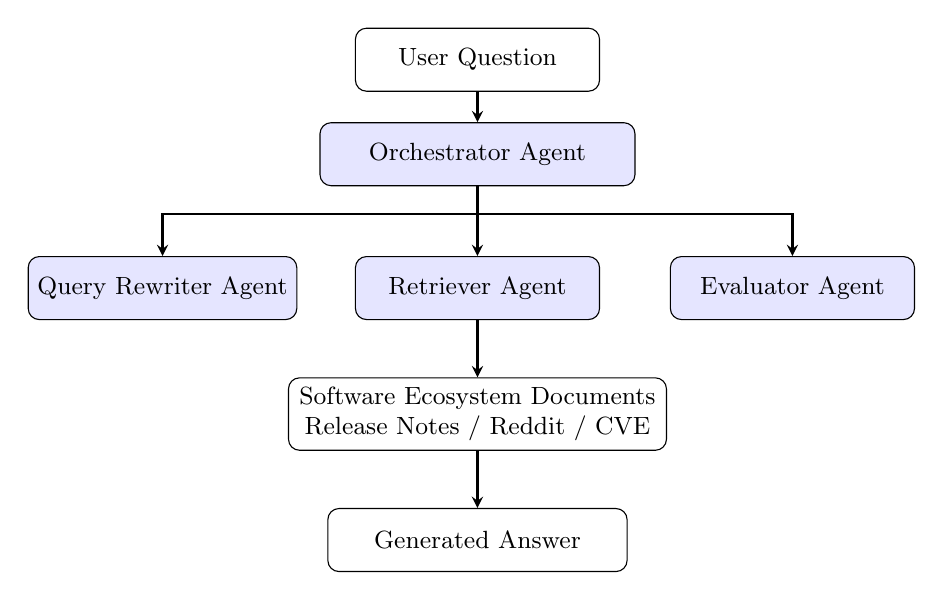
\begin{tikzpicture}[
  box/.style={
      rectangle,
      draw,
      rounded corners,
      text centered,
      align=center,
      minimum height=0.8cm,
      minimum width=3.1cm,
      font=\small,
      fill=white
  },
  agent/.style={
      box,
      fill=blue!10
  },
  arrow/.style={
      ->,
      thick,
      >=stealth
  }
]

% ==================================================
% User Query
% ==================================================

\node[box] (user) at (0,5.2)
      {User Question};

% ==================================================
% Orchestrator
% ==================================================

\node[agent,
      minimum width=4.0cm]
      (orch) at (0,4.0)
      {Orchestrator Agent};

% ==================================================
% Specialized Agents
% ==================================================

\node[agent]
      (rw) at (-4.0,2.3)
      {Query Rewriter Agent};

\node[agent]
      (ret) at (0,2.3)
      {Retriever Agent};

\node[agent]
      (eval) at (4.0,2.3)
      {Evaluator Agent};

% ==================================================
% Documents
% ==================================================

\node[box,
      minimum width=4.8cm]
      (docs) at (0,0.7)
      {Software Ecosystem Documents\\
       Release Notes / Reddit / CVE};

% ==================================================
% Answer
% ==================================================

\node[box,
      minimum width=3.8cm]
      (ans) at (0,-0.9)
      {Generated Answer};

% ==================================================
% Main Flow
% ==================================================

\draw[arrow]
      (user.south)
      -- (orch.north);

\draw[arrow]
      (orch.south)
      -- ++(0,-0.35)
      -| (rw.north);

\draw[arrow]
      (orch.south)
      -- (ret.north);

\draw[arrow]
      (orch.south)
      -- ++(0,-0.35)
      -| (eval.north);

\draw[arrow]
      (ret.south)
      -- (docs.north);

\draw[arrow]
      (docs.south)
      -- (ans.north);

\end{tikzpicture}%
}
\caption{Adaptive multi-agent RAG architecture.}
\Description{Block diagram of the adaptive multi-agent architecture. A user question enters an Orchestrator agent, which delegates to a Query Rewriter, a Retriever, and an Evaluator in sequence. The Retriever draws on software ecosystem documents comprising release notes, community discussions, and security advisories. The Evaluator scores retrieval quality and can return control to the Orchestrator to retry retrieval before an answer is generated.}
\label{fig:architecture}
\end{figure}

\subsection{Agent Definitions}\label{sec:agents}

The architecture comprises four agents organized under Orchestrator
coordination.

\textbf{Orchestrator Agent.}
The Orchestrator coordinates execution of the retrieval pipeline. It
receives the user question, delegates tasks to the remaining agents, and
manages retrieval retries when requested by the Evaluator. The
Orchestrator does not perform retrieval or answer generation directly.

\textbf{Query Rewriter Agent.}
The Query Rewriter addresses differences between user vocabulary and
document vocabulary. Llama~3.1~8B is used to transform the original
question into a retrieval-oriented representation. In the self-improving
configuration, learned terms from previous retrieval outcomes are
incorporated before query generation.

\textbf{Retriever Agent.}
The Retriever performs vendor-aware document retrieval. It first
attempts to identify the software vendor referenced in the query using
exact matching, alias lookup, and fuzzy matching against a registry of
software product names and subreddits fetched at startup (14,223 and 628
respectively when this was written; 1,348 and 364 as of 2026-09-23 --- see
Section~\ref{sec:datasources}). If a
vendor is detected, retrieval is restricted to vendor-specific
release notes, advisories, and community discussions. Otherwise, a
general retrieval logic is used. The Retriever returns ranked
documents without evaluating their quality \cite{guan2025, zheng2026, yang2026}.

\textbf{Evaluator Agent.}
The Evaluator estimates retrieval quality using a deterministic score
between 0.0 and 1.0. The score combines evidence from retrieval
volume, release-note matches, community matches, and CVE matches. If
the score falls below a predefined threshold, the Evaluator signals the
Orchestrator to perform an additional retrieval attempt. The released
implementation sets that threshold at $\theta = 0.15$; the earlier
evaluation harness, whose carried-over measurements
Section~\ref{sec:carried-over} reports, used $\theta = 0.30$. A second
constant of 0.30 appears in the same scoring method and is unrelated to the
retry decision: it is a quality floor applied when a Tier~1 or Apple source
is present. Since the fix described in Section~\ref{sec:retry}, the retry
signal is read from the overlap score before any such floor is applied, while
the floored score remains what is reported. The Evaluator does not generate
answers \cite{zhuge2024}.

\subsection{Adaptive Feedback and Self-Improvement}

The architecture incorporates a retrieval-level feedback loop. After
retrieval, the Evaluator assigns a quality score to the retrieved
documents. If retrieval quality is insufficient, the Orchestrator
re-executes the retrieval pipeline using a revised question generated by
the Query Rewriter.

The system also maintains a persistent Self-Improvement Memory. Query
expansion terms accumulate positive or negative scores based on
retrieval outcomes across sessions. Successful retrievals increase
associated term weights, while unsuccessful retrievals decrease them.
These scores are subsequently used by the Query Rewriter to influence
future retrieval queries. This mechanism provides adaptation without
human preference labels, manual annotation, or model retraining. It is
exercised by the earlier evaluation harness whose measurements
Section~\ref{sec:carried-over} reports, and not by the configuration measured
in Sections~\ref{sec:two-metrics}--\ref{sec:scaled-eval}; see
Section~\ref{sec:setup}.

\subsection{Software Ecosystem Data Sources}\label{sec:datasources}

The system retrieves information from software ecosystem documents
obtained through multiple API endpoints.

\textbf{Verified Sources}
\begin{itemize}
\item \texttt{/\{vendor\}}: vendor registry (6,578 entries)
\item \texttt{/v/}: software release notes (31,958 entries)
\item \texttt{/cve}: vulnerability advisories (24,139 entries)
\end{itemize}

\textbf{Community Sources}
\begin{itemize}
\item \texttt{/reddit}: community discussions (208,466 posts)
\item \texttt{/positive}: software update risk discussions (2,637 posts)
\item \texttt{/by-subreddit?q=\{vendor\}}: vendor-specific discussions
\item \texttt{/questions}: software-related user questions
\end{itemize}

To support vendor-aware retrieval, a registry of software vendors and
associated subreddits is loaded at startup and cached locally.

The entry counts above are those measured when the conference version was
written. They are not re-measurable: the endpoints return query results
without a collection total, so a reader cannot check them against the live
service. The one count that can be checked has moved substantially ---
\texttt{/api/c/names}, the product vocabulary the vendor matcher is built
from, returned 14,223 names then and returns 1,348 today (2026-09-23, full
response, not paginated). We report the original figures rather than silently
restate them, and note that any absolute corpus size in this section should be
read as a measurement of the service at that time rather than a stable
property of it. Retrieval results in this paper are unaffected: every run
either records its own corpus snapshot or is replayed from one
(Section~\ref{sec:tier-control}).

\subsection{Two Roles for a Rewritten Query}\label{sec:rewrite-roles}

A rewritten query serves two distinct purposes in a retrieval pipeline,
and the properties it needs for each are in tension. Issued to a
retrieval endpoint, its job is to \emph{widen} the candidate set:
vendor synonyms, product aliases, and the technical vocabulary of
release notes and advisories all admit documents the user's own
phrasing would not reach. Used to order that set, its job would be to
express what the user asked --- which by construction it no longer
does, having replaced the user's words with a paraphrase written for
the document collection.

The Query Rewriter is prompted for a retrieval-oriented restatement of
at most 20 words directed at bug fixes, releases, changelogs, security
patches, and performance. It therefore introduces terms frequent in the
collection and absent from the question, and drops terms rare in the
collection and decisive in the question. We expected both effects to raise
recall while lowering the precision of any ordering computed from the rewrite,
and on that expectation we adopt a single design rule and apply it throughout
the Retriever:

\begin{quote}
\emph{The rewritten query determines what is fetched. The original
question determines how it is ordered.}
\end{quote}

Let $q$ denote the user's original question and $\tilde{q}$ the
rewritten query returned by the Query Rewriter. The Retriever receives
both: candidate acquisition (Section~\ref{sec:union-fetch}) is
parameterized by $\tilde{q}$ and $q$ jointly, ranking
(Section~\ref{sec:rerank}) by $q$ alone. Two auxiliary decisions follow
the same rule. Vendor identification runs on $q$, because rewrites
reliably inject the tokens \texttt{release}, \texttt{update}, and
\texttt{fixes}, which the vendor registry matches as product names. The
gate on the model-release endpoint is evaluated on $q$ and $\tilde{q}$
concatenated, because a rewrite can drop the model name that made the
question a model question. Date extraction is the one place where the
implementation reads $\tilde{q}$ rather than $q$.

\subsection{Candidate Acquisition by Union Fetch}\label{sec:union-fetch}

Let $\mathcal{E}$ be the set of retrieval endpoints and $R_e(x)$ the
document list endpoint $e$ returns for a phrasing $x$. The Retriever
searches the phrasing set
\begin{equation}
Q =
\begin{cases}
\{\tilde{q}\} & \text{if } \mathrm{fold}(q) = \mathrm{fold}(\tilde{q}),\\
\{\tilde{q},\, q\} & \text{otherwise,}
\end{cases}
\label{eq:phrasings}
\end{equation}
where $\mathrm{fold}(\cdot)$ denotes whitespace-trimmed
lower-casing. The raw candidate multiset is the union
\begin{equation}
C = \bigcup_{e \in \mathcal{E}(q,\tilde{q})} \; \bigcup_{x \in Q} R_e(x),
\label{eq:union}
\end{equation}
in which $\mathcal{E}(q,\tilde{q}) \subseteq \mathcal{E}$ is the
endpoint subset admitted by the conditions in
Table~\ref{tab:endpoints}. Equation~\eqref{eq:phrasings} is what leaves
the single-agent baseline unaffected: the baseline passes the same
string as both original and rewritten, $Q$ collapses to one phrasing,
and Equation~\eqref{eq:union} reduces to the pre-existing
behavior. Section~\ref{sec:results} is therefore a before/after on the
multi-agent arm alone.

Documents from different phrasings and endpoints overlap heavily, so
$C$ is deduplicated by an identity function
\begin{equation}
\kappa(d) =
\begin{cases}
u(d) & \text{if } u(d) \neq \varepsilon,\\
\mathrm{fold}\big(\mathrm{title}(d) \,\|\, \mathrm{source}(d)\big) & \text{otherwise,}
\end{cases}
\label{eq:key}
\end{equation}
where $u(d)$ is the document's URL, $\varepsilon$ the empty string, and
$\|$ string concatenation. The URL is the reliable identifier. The
title-and-source fallback exists only for feeds that omit it and is
deliberately not the primary key, because titles repeat systematically
within a feed --- every CISA KEV row is formatted from one template.

Deduplication is order-preserving and runs per trust tier, with the
Tier~1 key set pre-seeded into the Tier~2 pass so that a document
reachable from both tiers appears only in the higher one:
\begin{equation}
P_1 = \mathrm{dedupe}(C_1), \qquad
P_2 = \mathrm{dedupe}\big(C_2 \,;\, \{\kappa(d) : d \in P_1\}\big),
\label{eq:tiers}
\end{equation}
where $C_1$ and $C_2$ are the verified and community subsets of $C$,
concatenated vendor-specific-first. The candidate pool is
$P = P_1 \frown P_2$, and $P$ itself is recorded per question, so that
``the reranker mis-ordered the document'' and ``the document was never
fetched'' remain separable diagnoses.

\begin{table}[t]
\caption{Retrieval endpoints, trust tier, how the phrasing enters the
request, and the condition for querying. \emph{Client-side} endpoints
retrieve a fixed feed and filter it locally by term overlap with the
phrasing; \emph{server-side} endpoints pass the phrasing as a request
parameter.}
\label{tab:endpoints}
\small
\footnotesize
\begin{tabular}{@{}p{0.26\linewidth}@{\hspace{6pt}}c@{\hspace{6pt}}p{0.30\linewidth}@{\hspace{6pt}}p{0.26\linewidth}@{}}
\toprule
Endpoint & Tier & Phrasing enters as & Queried when \\
\midrule
\texttt{/api/c/name/\{vendor\}}      & 1 & not used (vendor name only) & vendor detected ($\leq 2$ vendors) \\
\texttt{/api/v/}                     & 1 & client-side, overlap $\geq 2$ & vendor release lookup empty \\
Apple developer releases RSS         & 1 & client-side, overlap $\geq 1$ or Apple term & always \\
CISA Known Exploited Vulnerabilities & 1 & client-side, overlap $\geq 2$ & always \\
CIRCL Apple CVE Atom feed            & 1 & client-side, overlap $\geq 1$ & always \\
\texttt{/api/reddit/query/cve}       & 1 & server-side & always \\
\texttt{/api/v/search?q=}            & 1 & server-side, one request per term ($\leq 4$) & question mentions a model \\
\midrule
\texttt{/api/reddit/by-subreddit}    & 2 & client-side (\texttt{q} is the subreddit) & vendor detected ($\leq 3$ subreddits each) \\
\texttt{/api/reddit/query/positive}  & 2 & client-side, overlap $\geq 1$ & vendor subreddit search empty \\
Google News RSS search               & 2 & server-side, with appended terms & always \\
\bottomrule
\end{tabular}
\end{table}

Three endpoints are conditional. The general release feed is queried
only when the vendor-specific release lookup returned nothing, so a
recognized vendor suppresses it, and the general community feed is
queried only when the vendor subreddit search returned nothing. The
model-release endpoint is reachable only through a per-term search,
costing one request per query term, so it is gated on the question
plausibly concerning a model --- tested against a word-boundary
vocabulary of model names, model-shipping vendor brands, and generic
model terminology --- and capped at four terms issued concurrently. The
vendor release lookup is keyed on the extracted vendor name and is
issued once per vendor irrespective of $|Q|$; it is the one endpoint
the union does not duplicate.

\subsection{Reranking Against the Original Question}\label{sec:rerank}

Ranking is a separate, replaceable stage scored against $q$ when the
caller supplies it and against $\tilde{q}$ otherwise; every caller in
the pipeline supplies it. Let
$\tau(d)$ be the text a reranker sees: the concatenation of the
document title, its detail or body text, its top-voted community
comment where one was retrieved, and its subreddit. This is the same
text the answer synthesizer is shown, so ranking and synthesis cannot
disagree about what a document says. A reranker is a scoring function
$s(q, d)$; each tier is sorted by descending $s(q, \cdot)$, the sorted
tiers are concatenated, and the cut to the top $k$ documents ($k = 4$)
is applied once, at the end. Sorting within tier rather than over the
flat pool preserves the verified-before-community prior: lexical
scoring favors long community posts that repeat query terms, so a flat
sort can return a release question's top-$k$ as four community posts
and zero verified records. The sort is stable, so equal-scoring
documents retain their acquisition order.

Three backends are provided and selected by the environment variable
\texttt{MARAG\_RERANK}, so the choice is an ablation arm rather than an
assumption. Let $T(\cdot)$ denote the tokenizer, $D$ the set of
documents passed to the ranker (one trust tier), $N = |D|$,
$f(t,d)$ the frequency of token $t$ in $T(\tau(d))$,
$|d| = |T(\tau(d))|$, $\overline{L}$ the mean of $|d|$ over $D$, and
$n_t = |\{d \in D : t \in T(\tau(d))\}|$.

\textbf{\texttt{none}.} The published ranking function: a substring
boost on the head tokens of the ranking query,
\begin{equation}
s_{\mathrm{none}}(q, d) = \mathbf{1}\big[\exists\, w \in H(q) : w \sqsubseteq \mathrm{fold}(\mathrm{title}(d))\big],
\label{eq:none}
\end{equation}
where $H(q)$ is the first four whitespace-separated tokens of $q$ of
more than three characters and $\sqsubseteq$ is the substring
relation. Boosted documents are moved ahead of the rest and relative
order is otherwise preserved. This backend reproduces the scoring
function of the previously published configuration and is retained as
the ablation arm for the ranking stage. It is the function that is
reproduced, not the whole earlier configuration: the ranking query
supplied at the call site is now $q$, where the published pipeline
supplied $\tilde{q}$.

\textbf{\texttt{bm25}.} Okapi BM25 with the Robertson/Sp\"arck-Jones
defaults $k_1 = 1.5$ and $b = 0.75$:
\begin{equation}
s_{\mathrm{bm25}}(q, d) = \sum_{t \in T(q)} \mathrm{idf}(t) \cdot
\frac{f(t,d)\,(k_1 + 1)}{f(t,d) + k_1\left(1 - b + b\,\dfrac{|d|}{\overline{L}}\right)},
\label{eq:bm25}
\end{equation}
\begin{equation}
\mathrm{idf}(t) = \max\!\left(0,\; \ln \frac{N - n_t + 0.5}{n_t + 0.5}\right).
\label{eq:idf}
\end{equation}
The sum runs over the token sequence of $q$, so a term the user
repeated contributes once per occurrence. Two properties of
Equations~\eqref{eq:bm25}--\eqref{eq:idf} are specific to this setting.
First, $N$, $n_t$, and $\overline{L}$ are computed over $D$ --- the
tens of documents actually being ordered --- rather than over a global
corpus. The pool is what the ranking decision is made over, and scoring
against it keeps this arm dependency-free and deterministic, so a
reviewer can rerun it without a model. Second, the zero floor in
Equation~\eqref{eq:idf} is load-bearing at this scale: a term every
candidate shares carries $n_t = N$ and no discriminating information,
and without the floor its negative IDF would actively demote the
documents containing it.

The tokenizer matches lowercase alphanumeric runs joined by dots, so
version strings stay whole --- \texttt{6.18.21} is one token, not three
--- and a leading \texttt{v} immediately followed by a digit is
stripped, so a release note writing \texttt{v6.18.21} tokenizes
identically to the \texttt{6.18.21} a user typed. Version identity is
the most load-bearing match in this domain --- whether a document
concerns the version being asked about usually decides whether it is
relevant at all --- and that decision must not depend on the prefix
convention of the source that published it.

\textbf{\texttt{embed}.} Cosine similarity between query and document
embeddings,
\begin{equation}
s_{\mathrm{emb}}(q, d) = \frac{\phi(q) \cdot \phi(\tau(d))}{\lVert \phi(q) \rVert \, \lVert \phi(\tau(d)) \rVert},
\label{eq:embed}
\end{equation}
where $\phi$ is the \texttt{nomic-embed-text} embedding served locally
through Ollama, applied to the first 4{,}000 characters of its
input. The score is zero when either vector is empty, the dimensions
disagree, or either norm is zero. Embeddings are memoized per process,
and the reranker itself is constructed once per process: the same
documents recur across the retry loop and across systems sharing a
candidate pool, and building a reranker per retrieval discarded the
cache before it could be hit while paying an availability probe on
every question. The embedding model runs locally, so no closed-model
API is required to reproduce a run.

The embedding backend degrades honestly rather than silently. If no
embedding model answers the availability probe, it falls back to BM25
but reports its specification as \texttt{bm25(fallback from
embed:\textit{model})} and sets a \texttt{degraded} flag that the
Retriever propagates to the evaluation harness, so a results table
cannot attribute a lexical run to a semantic backend. An unknown
specification raises rather than defaulting, so a typo in an ablation
sweep fails loudly instead of quietly measuring the wrong arm. Because
the backend performs network calls at ranking time, it can also fail
after a successful probe; ranking then degrades to BM25 and, failing
that, to the Retriever's own acquisition order, so adding a ranking
stage does not make retrieval capable of raising.

\subsection{Retrieval Cost of the Union}\label{sec:retrieval-cost}

Equation~\eqref{eq:union} adds one request per phrasing-parameterized
endpoint admitted by Table~\ref{tab:endpoints}, and none for the vendor
release lookup, which is keyed on the vendor name. The union is
therefore slightly less than a doubling of retrieval calls. For a
question with no model mention and a recognized vendor whose lookups
return documents, the request count rises from 13 to 24; for a question
with no recognized vendor, from 7 to 14. An open model gate adds up to
4 concurrent per-term searches per phrasing on top of either figure. Under the reranking
functions available at the time of that measurement, no additional
language model calls are incurred: the Query Rewriter is
invoked once either way, and reranking is either arithmetic over the
pool or one local embedding call per distinct document. The grading
cascade of Section~\ref{sec:tier} changes this, and
Section~\ref{sec:efficiency} prices it.

On the ten-question ground-truth set, mean end-to-end latency is
approximately 23~s per question for the multi-agent pipeline against
approximately 12~s for the single-agent baseline. That gap is not
attributable to the union alone; it also covers the Query Rewriter's
generation call, the Evaluator's scoring pass, and any retrieval retry
the Evaluator triggers, none of which the baseline performs. The
defensible statement is narrower. The remedy for the fetch-time defect
costs roughly one additional set of retrieval calls per question, and
the multi-agent configuration as a whole reaches retrieval parity with
the baseline at approximately twice its latency.

\subsection{Answer Generation}

Retrieved documents are synthesized into a final answer using a
structured prompt. The prompt constrains generation to information
contained in retrieved sources and defines explicit behavior for
common retrieval outcomes.

The synthesis process follows six rules:

\begin{enumerate}
\item Summarize matching community discussions and associated comments.
\item Report version-specific information when present in release notes.
\item Explicitly state when retrieved sources do not directly answer the question.
\item Do not generate unsupported version numbers, fixes, or CVE identifiers.
\item Restrict claims to information contained in retrieved sources.
\item Report when no matching vendor-specific information is available.
\end{enumerate}

\subsection{A Multi-Ecosystem Benchmark}\label{sec:benchmark}

The evaluation in the conference version used 50 questions drawn from a single
community source, which is too few to separate an architectural effect from
noise and too narrow to say anything about ecosystems other than the ones those
questions happened to mention. We therefore constructed a larger benchmark, and
we describe its construction here in enough detail to expose its biases, because
a benchmark assembled by the authors of the system it evaluates warrants that
scrutiny.

\subsubsection{Construction}

The benchmark contains 500 questions arranged as a $24 \times 5$ grid of
software ecosystem by question category, filled to 20 or 21 questions per
ecosystem and exactly 100 per category. It was built in two stages from one
cache and one seed --- 300 questions first, then 500 --- and the selection is
greedy over deterministically ordered pools, so the 300 are a strict subset of
the 500; where a measurement below is reported at $n=300$, it is on that
subset. The 24 ecosystems span mobile and desktop
platforms (Apple iOS, Apple macOS, Android, Windows), four Linux distributions
(Ubuntu, Debian, Fedora, Arch) and the kernel itself, browsers (Firefox,
Chrome), container infrastructure (Docker, Kubernetes), language package
ecosystems (npm/Node, pip/Python, cargo/Rust), self-hosted and home applications
(Home Assistant, NAS/self-hosted, WordPress), databases (PostgreSQL, MySQL,
NoSQL), developer tooling, and LLM/AI model releases. The five categories are
releases, bugs, security, community, and general.

Every question is mined from live data rather than authored: 249 are verbatim
titles of real community posts, and 51 are generated from real release or
advisory records. No question is a template with a hand-written stem. The
builder draws from a pool of 9,923 community posts and the release and advisory
endpoints described in Section~\ref{sec:datasources}, and it is deterministic:
a fixed seed, an on-disk response cache, and an \texttt{--offline} mode that
replays the cache, so two runs of the builder produce byte-identical output.
Each record carries the endpoint and record type it came from, so mined and
generated questions remain distinguishable in any analysis.

\subsubsection{Two Upstream Data Defects}

Two properties of the upstream feeds would have injected false questions into
the benchmark had they been consumed naively. We report them because they are
properties of the public data sources rather than of our pipeline, and anyone
building on the same feeds will encounter them.

This is not an isolated quirk of one feed. Vulnerability-database metadata is
known to be noisy: affected-version and severity records in the NVD contain
substantial inaccuracy~\cite{croft2023dataquality,croft2022severity,anwar2022nvd},
and inconsistencies between advisory text and structured metadata have been
documented at scale~\cite{dong2019inconsistencies}. Downstream models trained on
such labels inherit the noise~\cite{chakraborty2022vulndetection}. What follows is
the form the problem takes in the feeds used here.

First, on advisory records the product field names the \emph{index token} under
which the advisory was filed, not the affected product. An advisory for ``Mocha
Telnet Lite for iOS 4.2'' is stored with product \texttt{iOS} and version
\texttt{4.2.0}; advisories concerning Velero are stored under
\texttt{Kubernetes}. Templating those fields directly yields questions such as
\emph{``Is iOS v4.2.0 vulnerable?''}, which assert a falsehood in the question
itself and would be scored against a system for failing to confirm it. The
builder instead parses the affected product and version out of the advisory
text, keeps a record only when the parsed product belongs to a tracked
ecosystem, and discards the rest: of 3,113 advisory rows, 548 parsed and 268
could be confidently attributed.

Second, a minority of records carry malformed dates (for example
\texttt{23.30.13102017} and \texttt{2025[29]0213}). Since date agreement is one
of the two decisive facts in this domain, these records are dropped rather than
normalized by guessing.

We also stopped trusting the feed's own topical flags. Its CVE-relatedness flag
fires on posts such as \emph{``Best budget AI subscription / API tokens?''}, so
it is used only to break ties within the security category rather than to assign
one.

\subsubsection{Ground Truth and Its Limits}

Of the 500 questions, 72 carry a reference answer (51 of the first 300), and
only those generated from release or advisory records do --- a community post
title states a question but does not come with an authoritative answer.
Ground-truth coverage is therefore concentrated in the releases and security
categories, and any correctness or hallucination measurement over this
benchmark is computed on that subset rather than on all 500 questions.

A community post title comes with something else: the URL of the post it was
taken from, which the live community feed the system retrieves from will return
as a document. Section~\ref{sec:leak} reports what that did to every retrieval
measurement and how the harness now excludes it; the benchmark file carries the
URL on every record so that the exclusion, and the post-hoc correction of runs
made without it, are reproducible.

This has a consequence for sampling that we did not anticipate and that a
reader reusing the benchmark should know. A subset selected to balance ecosystem
and category, without regard to ground truth, can leave almost none: our first
100-question stratified selection carried a reference answer on 2 questions. A
selection that prefers ground-truth records within each grid cell retains 28.
Reported retrieval metrics are unaffected --- they rest on pooled relevance
judgments, not reference answers --- but any answer-correctness figure requires
the second kind of selection, and we report retrieval and answer-faithfulness
results rather than correctness for this reason.

\subsubsection{Coverage Gaps}

One of the 120 grid cells (Arch $\times$ security) had no live candidate
available at build time. Rather than synthesize one, the builder logs the gap
and fills the category quota from other ecosystems, so the category totals hold
exactly while that single cell is empty. Nineteen product-name lookups returned
404 because the product is not in the vendor catalogue (npm, pip, cargo,
Synology, Home Assistant, NixOS, GitLab among them); this is a catalogue
coverage limitation rather than an endpoint failure, and the affected ecosystems
are represented through their community and release records instead.

\subsection{Experimental Setup}\label{sec:setup}

Three evaluation sets are used, and they answer different questions.
The \emph{original} set is 50 software update questions spanning security, bug,
release, community, and general maintenance topics; it is the set on which the
superseded bespoke score was measured (Section~\ref{sec:two-metrics}). The
\emph{ground-truth} set is 10 questions carrying reference answers, used for the
diagnostic measurements in Sections~\ref{sec:two-metrics}
and~\ref{sec:localizing} because relevance judgments and document-level counting
are tractable at that size. The \emph{benchmark} set is the 500 questions of
Section~\ref{sec:benchmark}, from which a 100-question subset balanced across
category and ecosystem carries the scaled evaluation
(Section~\ref{sec:scaled-eval}), the first 300 carry the large live run, and
all 500 carry the leak-free measurement (Section~\ref{sec:leak}). Sample sizes are stated with every reported
number, since they differ across these three. The local fallback dataset contains 324 Reddit
posts collected through the software ecosystem data lake and filtered
using minimum quality criteria of at least 10 comments, 3 author
replies, and a quality score of at least 0.30.

The single-agent baseline issues the user's question directly and performs
retrieval, evaluation, and answer generation within a single agent, without a
rewriting step, specialized agents, adaptive retry, or self-improvement memory.
It is the $\mathrm{fold}(q) = \mathrm{fold}(\tilde{q})$ case of
Equation~\eqref{eq:phrasings}, so the union of
Section~\ref{sec:union-fetch} leaves it unchanged. It
uses the same retrieval endpoints and answer synthesis prompt as the
proposed architecture, isolating the effect of architectural
decomposition.

Two capabilities of the architecture are outside what the multi-agent arm of
Sections~\ref{sec:two-metrics}--\ref{sec:scaled-eval} exercises, and we state
this rather than let the architecture description stand in for the measured
configuration. That arm runs the Query Rewriter, the Retriever, and the
Evaluator directly: the Orchestrator's retry loop
(Section~\ref{sec:agents}) is not invoked, and the Self-Improvement Memory is
not attached. The comparison those sections report is therefore between the
baseline and a memoryless, retry-free multi-agent pipeline, which is the
configuration the union-fetch finding concerns. The retry and the memory are
measured only where Section~\ref{sec:carried-over} says they are.

All experiments were performed using Llama~3.1~8B executed through
Ollama with temperature set to zero. The evaluation platform consisted
of Apple Silicon hardware with 24\,GB memory and Metal GPU
acceleration.

\subsection{How a Reported Number Is Produced}\label{sec:protocol}

Every retrieval number in Section~\ref{sec:results} is the mean over questions
of a per-question, per-arm quantity computed by one harness
(\texttt{eval\_harness/run\_eval.py}) in one pass. Because the arms differ in
what they fetch, and because an LLM supplies the relevance labels, the order in
which those steps happen decides what the number can be read to mean. We
therefore trace a single question end to end rather than name the metrics and
leave the protocol implicit.

\paragraph{1. The question.} A benchmark record carries an id, the question
text, its ecosystem and category, the endpoint and record type it was mined
from, and---for a community-mined question---the URL of the post whose title it
is. Every arm in the run receives the same question string.

\paragraph{2. Retrieval.} Each arm retrieves through the same
\texttt{RetrieverAgent} against the endpoints of
Section~\ref{sec:datasources}: the baseline on the question, the multi-agent
arm on the union of the question and its rewriting
(Section~\ref{sec:union-fetch}). Before any ranking, the record's own source
URL is struck from the candidate pool of \emph{every} arm
(Section~\ref{sec:leak}). A run reads its documents in one of two corpus
modes, and which one decides what its numbers can later be re-derived from. In
\emph{record} mode the endpoints are queried live and every response is written
to a snapshot directory; in \emph{replay} mode the fetch is served from that
directory, and in the \emph{strict} variant a document request the snapshot
does not hold aborts the run rather than quietly going live. Either way the
arms of a single run are compared against one corpus, which is what every
comparison in this paper rests on. Only replay makes a run reproducible
afterwards, and the asymmetry is worth stating precisely because it is easy to
assume otherwise: a snapshot holds one response body per request key, a live
feed answers the same key differently over the hours a 500-question run takes,
and the directory keeps the last of those answers. A record-mode run therefore
cannot be replayed back into itself. Replaying one of ours reproduced its
multi-agent arm's candidate pools on 1 of 12 questions, while two replays of a
single configuration agree on 12 of 12 and are byte-identical. Record-mode
numbers are internally valid and externally irreproducible; replay-mode numbers
are both. Where a table's arms come from different runs we say so, and we do
not read a difference between a live-recorded arm and a replayed one as an
effect of the architecture.

Retrieval also reads the clock, which a snapshot of HTTP responses does not
freeze: a question carrying \emph{latest} or \emph{last week} becomes a date
filter, so the same snapshot replayed a day later can admit a different set of
documents. A recording now stamps its directory with the date it was made and
a replay pins the process clock to that stamp, which removes the drift between
two runs made on different days; an explicitly set clock overrides it, and a
snapshot recorded before the stamp existed reports no recording date rather
than a guessed one.

\paragraph{3. Ranking and cut.} The candidate pool is ordered by the run's
ranking function and cut to $k=4$. Two settings decide the ordering and are
recorded per run: the scorer (BM25, embedding cosine, reciprocal-rank fusion,
or an LLM grading cascade) and whether the verified-source tier prior is
applied before it or not (Section~\ref{sec:rerank}). The top-$k$ list of
document ids is what the metrics see; the documents themselves are what the
answer is synthesized from.

\paragraph{4. Judging.} The judged pool for a question is the union of what
\emph{all} arms returned for it---optionally widened to everything they
considered, which is what makes pool recall computable. Each
(question,~document) pair is labelled once, by \texttt{llama3.1} at temperature
zero, on a graded scale: 2 highly relevant, 1 related, 0 irrelevant. The label
is keyed by a hash of the question text together with the document id and
cached on disk, so it is computed once and reused for every arm in the run and
for every later run that retrieves the same document for the same question. No
arm is scored against a private set of judgments, and no arm is penalized for a
document that only a competing arm surfaced.

\paragraph{5. Metrics.} From the ranked list and those labels:
nDCG@$k$ with gain $2^g-1$ and the standard $\log_2$ discount, its ideal
computed from the same per-question pool; Recall@$k$ over the relevant
documents in that pool; MRR on the first document with grade $\geq 1$. The
denominators are therefore \emph{pool-relative}. A system cannot be charged for
relevant documents no arm retrieved, which makes these numbers valid for the
paired within-run comparisons this paper draws and invalid as absolute values
to compare against published figures computed over a fixed judged corpus. We
state the pooling protocol with every absolute number for this reason, and
Section~\ref{sec:pool-demo} measures what ignoring it costs: two arms whose
retrieved lists are byte-identical, scored in pools of different width, differ
by $+0.055$ recall@5.

\paragraph{6. Answer scoring.} The same judge scores each arm's answer for
faithfulness to its own retrieved contexts and for answer relevance, each in
$[0,1]$, and for correctness against the reference answer on the questions that
carry one. Section~\ref{sec:metric-threat} states what an LLM judge scoring a
template against prose measures, and why the \texttt{marag\_llm} arm exists.

\paragraph{7. Cost.} The harness counts, per arm and per question, every model
call and every prompt and completion token the arm itself spent, attributed by
role---rewriting, ranking, synthesis---with the judge's own calls excluded, so
an accuracy difference between arms can be read against what it cost to obtain.

\paragraph{8. Statistics.} Arms are compared pairwise on the per-question
values, never on the difference of two means: the paired difference vector
feeds an exact two-sided Wilcoxon signed-rank test at the sample sizes where it
is exact, a percentile bootstrap 95\% confidence interval over question-level
differences (10{,}000 resamples, fixed seed), and a win/tie/loss count.
Families of comparisons carry a Holm correction.

\paragraph{9. What is left behind.} A run writes a directory
\texttt{results/run\_\textless epoch\textgreater\_\textless dataset
hash\textgreater/} holding: \texttt{config.json}, the arm configuration
actually used---ranking function, tier mode, own-post exclusion, corpus
snapshot statistics, agent-rules hash---read back from the objects the run
built rather than from the environment it was launched with;
\texttt{per\_query.jsonl}, one row per question per arm with the ranked
document ids, every metric, latency, model calls and tokens;
\texttt{qrels.json}, the labels used by \emph{this} run alone, so its numbers
recompute from its own artifacts without the accumulated cache;
\texttt{aggregate.csv} and \texttt{report.md}. Each table in
Section~\ref{sec:results} names the run id it was computed from. Two senses of
recovery apply to it, and they are not the same. Every metric recomputes from
that directory alone, for any run: the ranked document ids and the judgments
are both on disk, so a reader can re-derive the numbers, re-score them under a
different metric, or pool them with another run's judgments without touching
the endpoints. Re-executing the pipeline and arriving at the same ranked lists
is the stronger sense, and it holds for runs made in replay, not for runs made
in record mode against the live feeds.

\subsection{Arm Comparability and the Ablation Ladder}\label{sec:ladder}

Set side by side, the two arms do not hold the same capabilities. The
multi-agent arm rewrites the query, fetches both phrasings, scores its own
retrieval, and---in the full architecture---retries and accumulates memory; the
baseline does none of these. A reader is entitled to ask whether the two arms
are performing the same task at all, and if they are not, what a difference
between them measures.

The asymmetries are of two kinds, and only one of them is a defect. Query
rewriting, union fetch, and adaptive retry \emph{are} the treatment: they are
the independent variable, and removing them from the multi-agent arm would
leave nothing to evaluate. What makes their comparison sound is not symmetry of
capability but symmetry of everything else. Both arms retrieve from the same
endpoints through the same Retriever, cut to the same $k$, synthesize through
the same prompt with the same model, are scored by the same judge on the same
questions, and are compared pairwise within a single run so that corpus drift
cancels. The baseline is an ablation of the coordination layer, not a different
system.

The second kind of asymmetry is not part of the treatment and does leak into
measurement: the bespoke retrieval score of Section~\ref{sec:two-metrics} and
the answer rendering of Section~\ref{sec:scaled-eval}. The bespoke score is the
Evaluator's internal control signal---the same quantity that gates the
retry---and the baseline has no counterpart to it, so reporting it as the
comparison metric grades the treatment with its own ruler; Section~\ref{sec:metric-threat}
retires it for that reason. Answer rendering is neutralized rather than
defended, by the \texttt{marag\_llm} arm. Confounds of this kind must be
removed; treatment asymmetries must not be.

Removing them one at a time is what the ablation ladder in
Table~\ref{tab:ladder} does. Each rung differs from the one below it by exactly
one capability, so each adjacent pair is a single-factor comparison rather than
a comparison of two architectures. Rung A3 additionally runs the Evaluator, but
in a prose arm the Evaluator's output is only its quality score: it changes
neither the retrieved documents nor the answer, so A2 versus A3 isolates the
union fetch and nothing else.

\begin{table}[t]
\caption{The ablation ladder. Each rung adds one capability to the rung below,
so every adjacent pair is a single-factor comparison. A1g branches from A1
rather than continuing the chain: it adds question grounding \emph{without}
any coordination, which is what separates understanding the question from
coordinating agents. All rungs are now measured against a frozen corpus
(Table~\ref{tab:ladder-results}); A4 executed but cannot trigger, for the
structural reason given in Section~\ref{sec:retry}.}
\label{tab:ladder}
\begin{tabular}{llll}
\toprule
Rung & Arm & Capability added & Status \\
\midrule
A0 & \texttt{raw} & none (no retrieval) & Measured \\
A1 & \texttt{single\_agent} & retrieval on the user's question & Measured \\
A1g & \texttt{single\_agent\_grounded} & question grounding, no coordination & Measured \\
A2 & \texttt{rewrite\_only} & query rewriting & Measured \\
A3 & \texttt{marag\_llm} & union fetch over both phrasings & Measured \\
A4 & \texttt{marag\_llm\_retry} & Orchestrator retry & Could not trigger as run \\
A5 & \texttt{marag} & template rendering & Measured \\
\bottomrule
\end{tabular}
\end{table}

The same reasoning applies to rendering, which is not a property of the
multi-agent arm but a factor crossing it. Of the four cells of
rendering~$\times$~retrieval, three were populated in
Section~\ref{sec:scaled-eval}: baseline retrieval with prose
(\texttt{single\_agent}), multi-agent retrieval with prose
(\texttt{marag\_llm}), and multi-agent retrieval with a template
(\texttt{marag}). The format effect reported there is therefore an inference
across two arms rather than an estimated main effect. The fourth cell---baseline
retrieval rendered through the Evaluator's template---closes the design; it
requires no generation call, since the template is assembled deterministically
from the retrieved documents, and it is available in the released harness as
\texttt{single\_agent\_template}. With all four cells, rendering and retrieval
become main effects with an interaction term.

A2, A4, and the fourth cell are now measured, together with A1g, and
Section~\ref{sec:ladder-results} reports them. The run satisfies the constraint
this design imposes: because the retrieval endpoints are live, every arm
executed against a recorded corpus snapshot in replay, so the rungs differ by
capability and not by corpus drift. One constraint remains open. If the
Self-Improvement Memory is ever attached as a further rung, term-weight
learning makes each question's outcome depend on the questions preceding it;
per-question differences then cease to be exchangeable and the paired tests
used throughout this section no longer apply as written.

\section{Results}\label{sec:results}

This section presents the evaluation results of the proposed adaptive
multi-agent RAG architecture. The evaluation examines retrieval quality,
answer accuracy, adaptive feedback behavior, self-improvement
performance, representative examples, failure modes, and implementation
observations across the three evaluation sets of Section~\ref{sec:setup}.

\subsection{Two Metrics, Two Orderings}\label{sec:two-metrics}

We first report retrieval quality under the score used in the conference
version of this work, and then under standard information-retrieval metrics.
The two disagree, and the disagreement is the entry point to this section's
main result.

The bespoke score is a keyword- and source-overlap measure between the question
and the retrieved set, computed by the Evaluator agent
(Section~\ref{sec:method}). Under it, the multi-agent architecture improved on
the single-agent baseline in all five question categories, from 0.680 to 0.798
overall --- a 17.2\% relative improvement, with a paired $t$-test over the 50
evaluation queries yielding $t(49)=2.32$, $p=0.020$.

We then re-scored the same pipeline with nDCG@$k$, Recall@$k$, and MRR. Graded
relevance labels were pooled across systems: every document retrieved by any
system for a question was judged once, and the resulting label was reused for
every system that retrieved it, so no system is scored against a private set of
judgments. Table~\ref{tab:inversion} reports the result on the ten
ground-truth validation questions.

\begin{table}[t]
\caption{The same two systems under the paper's own retrieval-quality score and
under standard IR metrics. Bespoke score: $n=50$. IR metrics: $n=10$, pooled
graded relevance, judge \texttt{llama3.1}. The paired difference is
multi-agent minus baseline over the same questions; $p$-values are exact
two-sided Wilcoxon signed-rank, except the bespoke column, which is the paired
$t$-test over 50 questions reported in the conference version. Confidence
intervals are given in the text. The IR columns are reproduced by
\texttt{scripts/inversion\_stats.py}.}
\label{tab:inversion}
\begin{tabular}{lrrrr}
\toprule
System & bespoke score & nDCG@1 & nDCG@3 & MRR \\
\midrule
Single-agent baseline & 0.680 & \textbf{0.800} & \textbf{0.765} & \textbf{0.800} \\
Multi-agent           & \textbf{0.798} & 0.133 & 0.145 & 0.250 \\
\midrule
Paired difference & $+0.118$ & $-0.667$ & $-0.620$ & $-0.550$ \\
Exact $p$         & $0.020$ & $0.016$ & $0.016$ & $0.031$ \\
\bottomrule
\end{tabular}
\end{table}

The ordering reverses. A 17.2\% advantage on one metric coexists with roughly a
five-fold deficit on another, over the same questions, the same live corpus, and
the same retrieved documents. Because the bespoke score rewards overlap between
the question and the retrieved set without reference to whether a retrieved
document actually answers the question, it can be maximized by retrieving many
topically adjacent documents. Standard IR metrics, scored against judged
relevance, cannot be.

Ten questions is few enough that the deficit deserves a test rather than an
assertion, so we report exact ones. The multi-agent arm is worse on seven of the
ten questions and tied on the remaining three, never better
(Figure~\ref{fig:inversion-per-query}); the mean paired
nDCG@3 difference is $-0.620$ with a percentile bootstrap 95\% CI of
$[-0.865, -0.348]$, an exact two-sided Wilcoxon signed-rank $p$ of $0.016$, and
a standardized effect size $d_z = -1.39$. A sign-flip permutation test on the
mean difference gives the same $p$. The direction is consistent across every
metric we computed: nDCG@1 $-0.667$, nDCG@5 $-0.632$, MRR $-0.550$, Recall@5
$-0.550$, with $p \le 0.031$ throughout.

Two caveats bound what those numbers establish, and we state them because the
sample size makes both load-bearing. First, the Wilcoxon test discards tied
pairs, leaving seven; with seven nonzero pairs the smallest two-sided $p$ the
design can return is $2/2^{7} = 0.0156$. The observed $p$ \emph{is} that floor,
so the correct reading is that every non-tied question favours the baseline ---
the strongest signal obtainable at this $n$ --- and not that the evidence would
survive a stricter threshold. Second, the confidence intervals are wide: they
place the deficit somewhere between roughly a third and nine tenths of the
metric's range. They establish the sign and the order of magnitude of the
inversion, which is the claim this section makes, and they do not pin its
magnitude. The magnitude claim we do make quantitatively is the document count
in Section~\ref{sec:localizing}, which does not depend on an interval estimate.

A third caveat, learned after the table was made and larger than the other
two, is that the IR columns measure something the bespoke column does not: how
often a system retrieved the question's own source post. On these ten questions
the baseline placed that post in its top~3 for seven, the multi-agent arm for
none (Section~\ref{sec:leak}). With the own post struck from ranking and
judgments the same run reads nDCG@3 0.397 for the baseline against 0.263 for the
multi-agent arm --- the ordering survives, the factor of five does not. We
retain the table as the measurement that started the investigation, and read
its magnitude as mostly leak.

\begin{figure}[t]
\centering
\includegraphics[width=\columnwidth]{Figures/inversion-per-query.pdf}
\caption{The inversion at the level of individual questions, which the aggregate
in Table~\ref{tab:inversion} cannot show. One mark per evaluation question,
sorted: the multi-agent pipeline is worse on seven and tied on three, and no
question favours it. The three ties are drawn rather than dropped because they
are why the exact test has seven usable pairs, which fixes the smallest
attainable two-sided $p$ at $2/2^{7}=0.0156$. Regenerated from the run's
per-query rows by \texttt{scripts/paper\_figures.py}.}
\Description{Horizontal stem chart of the per-question nDCG@3 difference
between the multi-agent pipeline and the single-agent baseline, one stem per
evaluation question, sorted by that difference. Seven stems extend left of
zero, towards the side favouring the single-agent baseline, four of them
reaching the axis minimum of minus one; three questions are tied and appear as
open squares on the zero line; no stem extends right of zero. A dashed vertical
rule marks the mean difference of minus 0.620.}
\label{fig:inversion-per-query}
\end{figure}

\subsection{Localizing the Loss: Ranking or Retrieval?}\label{sec:localizing}

A deficit of this size has two candidate explanations. Either the pipeline
retrieves appropriate documents and orders them badly, or it does not retrieve
them. These call for different fixes, and they are indistinguishable from the
final top-$k$ alone.

The vocabulary-mismatch framing that motivates query rewriting in the literature
invites the first reading, and it is the one we pursued first. The retriever's
ordering was a substring boost computed over the first four tokens of the
rewritten query, which after a rewrite are typically filler
(Section~\ref{sec:rerank}). We replaced it with three progressively stronger
rerankers scored against the user's original question.
Table~\ref{tab:ranking-ablation} reports the outcome.

\begin{table}[t]
\caption{Ranking and retrieval ablation on the multi-agent arm ($n \le 10$).
Panel~(a): with only the rewritten phrasing retrieved, successively stronger
ranking functions raise MRR monotonically while nDCG@3 stays flat --- the
signature of a candidate set that does not contain the answer. Panel~(b): with
both phrasings retrieved and the pools merged, every configuration improves
sharply, and the choice of which phrasing to \emph{rank} against is worth far
less (0.597 versus 0.621) than the choice of which to \emph{retrieve} with.
Rows come from separate runs against live sources and are therefore not strictly
paired; the panel~(a)/(b) contrast is large enough to survive that, the
within-panel~(b) contrast is not.}
\label{tab:ranking-ablation}
\begin{tabular}{llrrr}
\toprule
Ranking function & Scored against & nDCG@3 & MRR & Recall@5 \\
\midrule
\multicolumn{5}{l}{\emph{(a) Single-phrasing retrieval: the rewritten query only}} \\
Substring boost & original question & 0.145 & 0.250 & 0.200 \\
Okapi BM25      & original question & 0.212 & 0.500 & 0.343 \\
Embedding cosine & original question & 0.188 & 0.625 & 0.327 \\
\midrule
\multicolumn{5}{l}{\emph{(b) Union retrieval: both phrasings issued, pools merged}} \\
Substring boost & rewritten query  & 0.597 & 0.650 & 0.650 \\
Substring boost & original question & 0.621 & 0.667 & 0.611 \\
Embedding cosine & original question & \textbf{0.765} & \textbf{1.000} & 0.165 \\
\bottomrule
\end{tabular}
\end{table}

Figure~\ref{fig:localization} plots both panels. Within panel~(a), MRR rises
monotonically from 0.250 to 0.625, confirming that
ranking was genuinely defective: better ranking does place better documents
first among those available. But nDCG@3 stays near 0.19 throughout. A ranking
intervention that improves ranking without closing the gap is evidence that the
gap is not a ranking problem.

\begin{figure}[t]
\centering
\includegraphics[width=\columnwidth]{Figures/localization.pdf}
\caption{Why the deficit is a retrieval problem and not a ranking one, from the
same runs as Table~\ref{tab:ranking-ablation}. Both measures share one axis. In
panel~(a) successively stronger ranking functions lift MRR from 0.25 to 0.62
while nDCG@3 stays between 0.14 and 0.21: the ranker is ordering a candidate set
that does not contain the answer. In panel~(b) the pools are unioned and both
measures move together, with the weakest ranking function already reaching 0.60.
The panels differ only in which phrasing was \emph{retrieved}, which is why the
split is the layout rather than a series.}
\Description{Two panels sharing a vertical axis, each plotting mean
reciprocal rank alongside nDCG at 3 for successively stronger ranking
functions. In panel (a), single-phrasing retrieval, MRR rises from 0.25 to
0.62 while nDCG at 3 stays flat between 0.14 and 0.21, so the two measures
diverge. In panel (b), union retrieval, both measures rise together and the
weakest ranking function already reaches 0.60.}
\label{fig:localization}
\end{figure}

Panel~(b) makes the same point from the other direction, and also bounds our own
claim. Once both phrasings are retrieved, even the original substring boost ---
the weakest ranking function available, and the one the pipeline shipped with
--- reaches nDCG@3 of 0.597, four times its panel~(a) value. Ranking the merged
pool against the original question rather than the rewrite adds 0.024 on top of
that (0.621 versus 0.597), a difference we do not regard as established at this
sample size. In other words: of the two changes we made, the one we made first
and reasoned about most carefully --- ranking against the user's question ---
turns out to matter far less than simply retrieving with both phrasings. We
report this because it is the opposite of the order in which we found it, and
because a reader deciding what to adopt should adopt the union first.

We therefore stopped inferring from scores and counted documents directly. For
each question we took the documents the single-agent baseline retrieved that the
judge had labelled relevant, and asked whether each appeared anywhere in the
multi-agent pipeline's retrieved set:

\begin{quote}
Of the 23 relevant documents the single-agent baseline retrieved across the
evaluation set, \textbf{22 were never retrieved by the multi-agent pipeline at
all.}
\end{quote}

The cause is a wiring property rather than a modelling one. Every retrieval
endpoint was being issued the rewritten query \emph{instead of} the user's
question. The rewrite is a lossy paraphrase --- it is designed to be, since its
purpose is to substitute domain vocabulary for user vocabulary --- and the
documents matching the user's own phrasing were consequently never candidates.
No reranker can promote a document that was never retrieved, which is precisely
what Table~\ref{tab:ranking-ablation} shows.

The remedy follows directly and is stated in Section~\ref{sec:union-fetch}: issue
both phrasings and union the candidate pools. The final row of
Table~\ref{tab:ranking-ablation} gives its effect --- nDCG@3 from 0.188 to 0.765
in a single change, with no modification to ranking, generation, or the
evaluator. Notably, the multi-agent pipeline had all along been retrieving
relevant documents the baseline missed; its candidate set was not worse so much
as \emph{different and smaller}, which is why unioning rather than replacing
recovers the loss.

What it recovers is the question. Every row of Table~\ref{tab:ranking-ablation}
was re-scored with the question's own source post struck from the ranked list
and from the judgments (Section~\ref{sec:leak}). In panel~(a) the embedding row
reads 0.309 leak-free rather than 0.188; in panel~(b) it reads 0.216 rather than
0.765, with the own post present in all ten of its top-3 lists. The union fetch
did not move the pipeline from 0.188 to 0.765 on documents that answer the
question; it moved it from 0.309 to 0.216 on those, and restored the one
document that matched the user's wording exactly because it was the user's
wording. The 22 of 23 count is a census and still stands as one; what it counted
was, for the most part, source posts.

\subsubsection*{The divergence signature disappears once the defect is repaired}

Table~\ref{tab:ranking-ablation} carries two weaknesses that the diagnosis rests
on and that ten questions cannot remove: its rows come from separate runs against
live sources, so they are not strictly paired, and the pattern it reports could in
principle be an artifact of the sample. We therefore repeated the ranking
ablation on the repaired pipeline over the 100-question benchmark, against a
corpus snapshot recorded once and then replayed, so that the three arms differ
only in the ranking function and every arm sees byte-identical documents.
Table~\ref{tab:scaled-ablation} reports it.

\begin{table}[t]
\caption{Ranking ablation repeated on the repaired pipeline, $n=100$, against a
frozen corpus snapshot replayed identically for all three arms
(\texttt{corpus\_misses}~$=0$, \texttt{frozen}~$=$~true). Unlike
Table~\ref{tab:ranking-ablation} these rows are strictly paired. With the union
fetch in place, stronger ranking now moves nDCG@3 and MRR \emph{together} ---
the divergence that localized the defect is absent, which is what the diagnosis
predicts. Levels in this table are inflated by the own-post leak of
Section~\ref{sec:leak} (72--73\% of top-$k$ lists on this frozen corpus); the
within-table contrasts, which compare arms that leak at the same rate, are what
it is cited for.}
\label{tab:scaled-ablation}
\begin{tabular}{llrrrr}
\toprule
Ranking function & System & nDCG@3 & nDCG@5 & MRR & Recall@5 \\
\midrule
None            & multi-agent  & 0.486 & 0.473 & 0.618 & 0.341 \\
                & single-agent & 0.507 & 0.493 & 0.646 & 0.371 \\
Okapi BM25      & multi-agent  & 0.627 & 0.596 & 0.793 & 0.387 \\
                & single-agent & 0.631 & 0.606 & 0.806 & 0.396 \\
Embedding cosine & multi-agent  & \textbf{0.656} & \textbf{0.615} & \textbf{0.817} & 0.387 \\
                 & single-agent & 0.646 & 0.612 & 0.808 & 0.388 \\
\bottomrule
\end{tabular}
\end{table}

The contrast with panel~(a) is the point. There, three successively stronger
ranking functions raised MRR by 0.375 while leaving nDCG@3 within 0.043 of where
it started: ranking was working and the answer was not in the candidate set to be
ranked. Here the same progression raises nDCG@3 by 0.170 and MRR by 0.198 on the
multi-agent arm --- the two measures move together, which is what ranking
improvements look like when the candidate set does contain the answer. A
diagnosis of the form ``this metric pattern indicates a fetch defect rather than
a ranking defect'' is falsifiable in exactly this way, and the pattern is absent
once the fetch is repaired.

Two further readings are available from the same table. The candidate-pool
ceiling separates the two systems consistently --- mean pool recall 0.981 for the
multi-agent arm against 0.839 for the single-agent baseline, stable across all
three ranking functions --- so the union fetch does raise the ceiling reranking
can reach, which is the mechanism Section~\ref{sec:union-fetch} claims. And the
choice of ranking function matters more than the choice of architecture at this
scale: moving from no reranking to embedding cosine is worth 0.170 nDCG@3, where
the gap between the two architectures under any fixed ranking function never
exceeds 0.021.

\subsection{Evaluation at Scale}\label{sec:scaled-eval}

The preceding measurements use ten ground-truth questions and are diagnostic
rather than conclusive. To test whether the repaired pipeline holds up, we
evaluated on a 100-question stratified subset of the 300-question benchmark
(Section~\ref{sec:benchmark}), balanced across all five question categories at 20
each and covering 21 of the 24 software ecosystems. All 100 questions completed
across all three systems.

Three systems were run with the synthesis model held constant at Llama 3.1 8B,
which isolates architecture from model:

\begin{itemize}
  \item \textbf{marag} --- the multi-agent pipeline as described, whose answer is
  a template assembled by the Evaluator agent from the retrieved documents.
  \item \textbf{marag\_llm} --- identical retrieval, but the answer is
  synthesized in prose through the same prompt the baseline uses. This arm
  exists solely so that answer-quality scores are comparable.
  \item \textbf{single\_agent} --- the baseline: raw query, one retrieval pass,
  one synthesis call.
\end{itemize}

\begin{table}[t]
\caption{Retrieval quality on the 100-question stratified benchmark subset
($n=100$), pooled graded relevance, judge \texttt{llama3.1}, mean $\pm$ 95\%
CI. Every arm was served from a corpus snapshot recorded in a preceding pass
and replayed here, so all three saw byte-identical documents: 6{,}348 snapshot
hits, and none of the misses on a document host. The two multi-agent arms are
configured identically and differ only in answer synthesis; under the frozen
corpus their ranked top-$k$ sets and their candidate pools now coincide on all
100 questions, as ordered lists and as sets, with no question excluded. The
earlier live-endpoint measurement of this table agreed on top-$k$ but on pools
only on 88 of the 93 questions where a pool existed --- that residual was
endpoint variability between two arms querying live, not a difference between
the systems, which is what freezing the corpus establishes. \emph{These levels
are not retrieval quality:} the question's own source post is in the top-$k$
list of every arm on 98 of the 100 questions and is the only judged-relevant
document for 58. Leak-free (Section~\ref{sec:leak}) the three rows read nDCG@3
0.320 / 0.320 / 0.331. The parity the table shows is real; its height is the
leak.}
\label{tab:scaled-retrieval}
\begin{tabular}{lrrrr}
\toprule
System & nDCG@3 & nDCG@5 & MRR & Recall@5 \\
\midrule
marag         & 0.922 $\pm$ 0.040 & 0.927 $\pm$ 0.038 & 0.945 $\pm$ 0.041 & 0.929 $\pm$ 0.039 \\
marag\_llm    & 0.922 $\pm$ 0.040 & 0.927 $\pm$ 0.038 & 0.945 $\pm$ 0.041 & 0.929 $\pm$ 0.039 \\
single\_agent & 0.924 $\pm$ 0.039 & 0.933 $\pm$ 0.037 & 0.948 $\pm$ 0.039 & 0.937 $\pm$ 0.038 \\
\bottomrule
\end{tabular}
\end{table}

Table~\ref{tab:scaled-retrieval} reports retrieval quality. The repaired
multi-agent pipeline and the single-agent baseline are indistinguishable: every
difference is well within overlapping confidence intervals, and the baseline is
nominally ahead on all four metrics. The fetch-time diagnostic of Section~\ref{sec:localizing} --- the share of the
baseline's relevant documents absent from the multi-agent \emph{candidate pool}
--- stands at 22 of 23 on the ten ground-truth questions and at \textbf{13 of
172 (7.6\%)} here, recomputed on the frozen corpus. The two figures come from
different question sets rather than from recomputing one on the other, but they
are the same measurement. Both, we now know, count mostly source posts
(Section~\ref{sec:leak}): the union fetch's effect on this diagnostic is that
the multi-agent pool once again contains the question.

These figures supersede an earlier measurement of the same comparison, and the
difference is worth stating because it is large. The release-fetching path
truncated its candidate list to the requested limit \emph{before} applying the
ranking function meant to demote advisory records, so for any product with an
active CVE feed the shipped releases were unreachable: a query for
\texttt{linux} returned no shipped release at all within forty retrieved
documents. Measured on that retriever, this table read nDCG@3 0.859 / 0.859 /
0.863 against the 0.922 / 0.922 / 0.924 reported here --- roughly six points of
retrieval quality that the defect, not the architecture, was costing. Both arms
called the same retriever, so the ordering was never affected; only the level
was. The same repair and the same frozen-corpus protocol are applied to
Table~\ref{tab:gt-run}.

\begin{table}[t]
\caption{Answer quality and cost ($n=100$), LLM-judged, mean $\pm$ 95\% CI.
\texttt{marag} and \texttt{marag\_llm} share a retrieval pipeline and differ
only in how the answer is produced. Quality is measured on the frozen-corpus
replay; latency is the per-question median from the live recording pass that
produced that snapshot, since a replay reads its documents from cache and its
timings measure nothing.}
\label{tab:scaled-answer}
\begin{tabular}{lrrr}
\toprule
System & Faithfulness & Answer relevance & Latency (s) \\
\midrule
marag (template answer)   & 0.748 $\pm$ 0.036 & 0.995 $\pm$ 0.004 & 18.8 \\
marag\_llm (prose answer) & 0.919 $\pm$ 0.035 & 0.968 $\pm$ 0.027 & 24.7 \\
single\_agent             & 0.929 $\pm$ 0.032 & 0.973 $\pm$ 0.021 & 8.4 \\
\bottomrule
\end{tabular}
\end{table}

\subsubsection{A Second Sample, and Why It Matters}

The 100-question subset above balances category and ecosystem without regard to
reference answers, which as Section~\ref{sec:benchmark} explains leaves almost
none. We therefore repeated the evaluation on a second 100-question selection
that prefers ground-truth records within each grid cell, retaining 28. This
permits an answer-correctness measurement, and it provides an independent sample
of the architecture comparison.

\begin{table}[t]
\caption{The same three systems on a second 100-question selection, one that
retains 28 reference answers, under the same frozen-corpus protocol (6{,}227
snapshot hits, no miss on a document host). Values are mean $\pm$ 95\% CI;
correctness is computed only where a reference answer exists, with $n$ given
per arm; latency is the median from the live recording pass. The nominal
ordering on retrieval is the reverse of Table~\ref{tab:scaled-retrieval}, and
remains so after the repair --- which is the point of reporting this sample.
Retrieval levels carry the own-post leak (72--73\% of top-$k$ lists; leak-free
nDCG@3 0.330 / 0.330 / 0.333).}
\label{tab:gt-run}
\begin{tabular}{lrrrr}
\toprule
System & nDCG@3 & Faithfulness & Correctness & Latency (s) \\
\midrule
marag         & 0.795 $\pm$ 0.071 & 0.735 $\pm$ 0.037 & 0.324 $\pm$ 0.109 ($n=27$) & 16.2 \\
marag\_llm    & 0.795 $\pm$ 0.071 & 0.939 $\pm$ 0.030 & 0.392 $\pm$ 0.160 ($n=25$) & 16.5 \\
single\_agent & 0.773 $\pm$ 0.075 & 0.932 $\pm$ 0.031 & 0.363 $\pm$ 0.134 ($n=27$) & 8.2 \\
\bottomrule
\end{tabular}
\end{table}

Table~\ref{tab:gt-run} is the most useful evidence in this section, for a reason
that has nothing to do with which system is ahead. On this sample the
multi-agent arm is nominally ahead on retrieval (0.781 versus 0.768), on
faithfulness once format is matched (0.938 versus 0.917), and on correctness
(0.367 versus 0.326). On the sample of Table~\ref{tab:scaled-retrieval} it was
nominally behind on all of them. Every one of these differences sits inside
overlapping confidence intervals in both runs. Two independent 100-question
samples that disagree about the direction of the difference are stronger
evidence that no difference is being measured than either sample is on its own,
and we read the pair that way rather than selecting the favourable one.

A caveat applies to both samples equally. Neither run uses a frozen corpus
snapshot --- the retrieval endpoints are queried live, and their contents change
between runs --- so the two samples are independent draws from a moving
distribution rather than a controlled replication. This is what makes the
direction reversal informative rather than contradictory: two draws that
disagree about the sign of a difference, each with intervals spanning zero, are
consistent with there being no difference to find. A frozen snapshot would be
required to make a positive claim about the size of one, and the harness
supports recording and replaying one for that purpose.

Three further observations. First, correctness is low for every arm --- between
0.30 and 0.37 --- so on version-specific questions with a checkable answer, all
three systems are wrong more often than right; retrieval parity should not be
mistaken for adequacy. Second, the correctness sample sizes differ across arms
(24 to 27) because an arm that abstains on a question yields no scoreable
prediction, which is itself informative and is why the CRAG-style scoring treats
abstention and error asymmetrically. Third, latency is not comparable between
the two tables: this run shared the machine with other work, so its absolute
figures are inflated. The within-run ratio --- roughly three times the
baseline's median here, twice it in Table~\ref{tab:scaled-answer} --- is the
quantity to read.

Table~\ref{tab:scaled-answer} carries a methodological result worth stating
separately. Comparing \texttt{marag} against \texttt{single\_agent} on
faithfulness suggests a substantial deficit (0.748 versus 0.929). Comparing
\texttt{marag\_llm} against \texttt{single\_agent} --- the same retrieval, the
same documents, differing only in whether the answer is a structured template or
model prose --- gives 0.919 versus 0.929. The apparent deficit was almost
entirely an artifact of answer \emph{format}: an LLM judge scoring a structured
template against fluent prose is partly scoring fluency. Any evaluation
comparing an agentic system that emits structured output against a baseline that
emits prose is exposed to this, and we would not have detected it without an arm
constructed specifically to remove it.

On cost, the multi-agent pipeline takes roughly twice to three times the median
per-question latency of the baseline (18.8\,s for the template arm and
24.7\,s for the prose arm, against 8.4\,s). This reflects the
rewriter's generation call, the evaluator pass, and the additional retrieval
calls the union incurs.

\subsection{The Complete Ladder}\label{sec:ladder-results}

Section~\ref{sec:ladder} set out the ladder as a protocol and reported three of
its rungs. We now run all of them, against a corpus frozen for the purpose, and
add the rung the protocol was missing.

Every arm answered the same 100 questions with synthesis held at
\texttt{mistral} wherever a generation call occurs, reranking at
\texttt{embed:nomic-embed-text}, and judging by
\texttt{qwen2.5:7b-instruct}, a model that wrote none of the answers. The
documents were served from a snapshot recorded in a preceding pass: 12,344
snapshot hits against 240 misses, none of the misses on a document host, so
every arm saw byte-identical documents. This is the strict-replay condition
Section~\ref{sec:ladder} required, and it is the same protocol under which
Tables~\ref{tab:scaled-retrieval} to~\ref{tab:gt-run} are now reported.

\begin{table}[t]
\caption{Every rung of the ladder on the 100-question benchmark, against a
frozen corpus. A4 reproduces A3 to three decimals on every metric because its
retry never triggered. A0 retrieves nothing, so its faithfulness has no
retrieved documents to be unfaithful to and is not comparable to the rest of
the column. Retrieval levels carry the own-post leak (Section~\ref{sec:leak}):
the source post is in 72--73\% of top-$k$ lists for every arm except A2, where
it is in 4\%. Leak-free nDCG@3: A1 0.269, A1g 0.321, A2 0.263, A3--A5 0.267.}
\label{tab:ladder-results}
\begin{tabular}{llrrrrr}
\toprule
Rung & Arm & nDCG@3 & nDCG@5 & MRR & Recall@5 & Faithfulness \\
\midrule
A0  & \texttt{raw}                   & ---   & ---   & ---   & ---   & 0.838 \\
A1  & \texttt{single\_agent}         & 0.731 & 0.742 & 0.806 & 0.731 & 0.750 \\
A1g & \texttt{single\_agent\_grounded} & \textbf{0.780} & \textbf{0.784} & 0.828 & \textbf{0.767} & 0.768 \\
A2  & \texttt{rewrite\_only}         & 0.210 & 0.231 & 0.352 & 0.301 & 0.785 \\
A3  & \texttt{marag\_llm}            & 0.752 & 0.761 & 0.822 & 0.738 & 0.754 \\
A4  & \texttt{marag\_llm\_retry}     & 0.752 & 0.761 & 0.822 & 0.738 & 0.754 \\
A5  & \texttt{marag}                 & 0.752 & 0.761 & 0.822 & 0.738 & 0.659 \\
2$\times$2 & \texttt{single\_agent\_template} & 0.731 & 0.742 & 0.806 & 0.731 & 0.648 \\
\bottomrule
\end{tabular}
\end{table}

Because the arms are paired within the run, the aggregate means understate what
is available: the per-question differences can be tested directly.
Table~\ref{tab:ladder-paired} reports them under a Wilcoxon signed-rank test.

\begin{table}[t]
\caption{Paired per-question differences, Wilcoxon signed-rank. ``Better'' and
``worse'' count the questions on which the second arm beat or lost to the
first; the remainder tie. Rows marked $\dagger$ report a $p$ below the smallest
value the test can attain at that number of non-zero pairs (0.0625 at five
pairs, 0.25 at three): they are null, not significant.}
\label{tab:ladder-paired}
\begin{tabular}{llrrrl}
\toprule
Comparison & Metric & Mean $\Delta$ & Better & Worse & $p$ \\
\midrule
A1 $\to$ A1g  & nDCG@3   & $+0.049$ & 14 & 5  & \textbf{0.0070} \\
A1 $\to$ A1g  & Recall@3 & $+0.051$ & 12 & 4  & \textbf{0.0035} \\
A1 $\to$ A1g  & nDCG@5   & $+0.042$ & 15 & 9  & \textbf{0.0268} \\
A1 $\to$ A1g  & Recall@5 & $+0.037$ & 13 & 9  & 0.0534 \\
A1 $\to$ A1g  & MRR      & $+0.023$ & 5  & 0  & 0.0431$^\dagger$ \\
A1 $\to$ A1g  & nDCG@1   & $+0.027$ & 3  & 0  & 0.1088$^\dagger$ \\
\midrule
A1 $\to$ A3   & nDCG@5   & $+0.018$ & 9  & 10 & 0.8721 \\
A1 $\to$ A3   & Recall@5 & $+0.007$ & 6  & 8  & 1.0000 \\
A1 $\to$ A3   & MRR      & $+0.016$ & 4  & 4  & 0.4838 \\
\midrule
A1g vs.\ A3   & nDCG@5   & $-0.024$ & 12 & 20 & 0.2172 \\
\bottomrule
\end{tabular}
\end{table}

Four results follow, and three of them change what the earlier sections can
claim.

\textbf{Coordination shows no retrieval benefit.} A1~$\to$~A3 is null on every
metric: nine questions better, ten worse, $p=0.87$ on nDCG@5 and $p=1.00$ on
Recall@5. This is not a small effect the sample was too thin to resolve; it is
the absence of one, and it agrees with the live-endpoint result of
Table~\ref{tab:scaled-retrieval} under a condition that removes corpus drift as
an explanation.

\textbf{Grounding the question may.} A1~$\to$~A1g is significant at $k=3$ and
$k=5$ as tabulated, and the gain is concentrated in the \texttt{releases}
category (nDCG@1 0.567 to 0.700), which is where the record-type confusion of
Section~\ref{sec:datasources} does its damage. Leak-free the gain is $+0.052$
nDCG@3 (13~better, 7~worse) and does not survive correction across the 21
comparisons the leak-free re-scoring runs; it wants a pre-registered test of its
own before it is quoted. The comparison A1g versus A3 is unaffected in
direction: a single agent that understands the question is statistically
indistinguishable from the full pipeline ($p=0.22$).

\textbf{The Orchestrator's retry never triggered.} A4 returned identical
documents \emph{and} identical answers to A3 on all 100 questions. The retry
fires when the Evaluator's quality score falls below 0.15; the minimum observed
across the benchmark was 0.300. Rung A4 is therefore reported as executed and
never triggered rather than as measured with no effect. Section~\ref{sec:retry}
returns to it at 500 questions and shows the gap is structural rather than a
property of these questions.

\textbf{Rewriting alone loses the source post, and the union is what
restores it.} A2 scores nDCG@5 0.231 against A1's 0.742, and A3 adds the union
and returns to 0.761, level with the baseline. When the first version of this
paper reported that row, it read it as rewriting collapsing retrieval and the
union repairing the collapse. It is not that. The question's own source post is
in A1's top-$k$ on 72 of 100 questions and in A2's on 4: a rewritten query no
longer matches the post's title verbatim, so the feed no longer returns it.
With the own post struck from ranking and judgments (Section~\ref{sec:leak}),
A2 reads nDCG@3 0.263 against A1's 0.269 --- a paired difference of $-0.006$,
8~questions better and 9~worse --- and Recall@5 is $+0.032$ in A2's favour. The
ladder's most dramatic contrast, 0.21 against 0.73, is the leak; leak-free,
rewriting alone is level with issuing the question verbatim, and the union fetch
adds nothing measurable to either.

Finally, the fourth cell of the rendering~$\times$~retrieval design is now
populated, and rendering is estimable as a main effect rather than inferred
across two arms. Template rendering costs approximately 0.10 faithfulness in
both cells: $-0.095$ from A3 to A5 (51 questions worse, 19 better) and $-0.102$
from A1 to \texttt{single\_agent\_template} (52 worse, 13 better), both
$p<0.0001$. The effect is the same magnitude under either retrieval pipeline,
which confirms it as a property of the rendering and not of the architecture.
Any comparison that places a template arm against a prose arm measures this
before it measures retrieval.

\subsection{The Own-Post Leak}\label{sec:leak}

Everything above this point was measured on a corpus that contained the
questions. This section reports how we found that out, how much of each
preceding table it accounts for, and what the comparison looks like with it
removed.

\subsubsection{How it surfaced}

To extend the 300-question run of Section~\ref{sec:scaled-eval} we built a
500-question benchmark by the same procedure, from the same cache and seed, so
that the 300 questions are a strict subset of the 500, and ran the same three
arms with the same judge, reranker, and configuration. On the 300 shared
questions the baseline's nDCG@3 fell from 0.818 to 0.494, and the multi-agent
arm's from 0.827 to 0.483. Nothing in the pipeline had changed. A uniform drop of
0.33 on every arm, on identical questions, is not a systems effect, and looking
for its cause exposed why the numbers had been high in the first place.

\subsubsection{Mechanism}

Of the benchmark's questions, 445 of 500 are the titles of real community
posts, and each carries the URL of the post it was taken from. The system
retrieves, among other sources, from the live feed those posts were mined from.
The feed returns the post the title came from; the harness derives the
document's identifier from its URL, so it is the same document the benchmark
record points to; and the relevance judge, asked whether a document is relevant
to a question, correctly marks the document that \emph{is} the question as
relevant. In the 300-question run the question's own post was in the candidate
pool for 247 of the 262 community-mined questions, was judged relevant for 232,
and was the \emph{only} judged-relevant document for 140. By the time of the
500-question run, two weeks later, the feed had aged past most of those posts:
171 of 445 in the pool, the only relevant document for 82. The score fell with
the leak.

The leak has a property that made it hard to see. Every arm that issues the
user's phrasing retrieves the own post at the same rate --- 72--73\% of top-$k$
lists on the frozen 100-question corpus, 82--83\% on the live 300, 98\% on the
frozen scaled-evaluation replay --- so the paired differences between such arms,
which is what every statistical test in this paper computes, never contained
it. It appears only in the absolute level, and only if the level is compared
across runs, which the frozen-corpus protocol we adopted for comparability
specifically discourages. The one arm that does \emph{not} issue the user's
phrasing is the rewrite-only arm, and it retrieves the own post 4\% of the time;
that is the whole of the 0.21-against-0.73 contrast in
Table~\ref{tab:ladder-results}.

\subsubsection{Post-hoc correction}

A script strikes the question's own post from each arm's ranked list and from
the judgments before recomputing the metrics. Table~\ref{tab:leak} applies it
to every retrieval table above.

\begin{table}[t]
\caption{Each retrieval measurement in this paper, as reported and with the
question's own source post struck from ranking and judgments. ``Own post in
top-$k$'' is the share of the arm's ranked lists containing it. Leak-free, every
arm at every sample size lies between 0.26 and 0.34, and the arms that leak at
the same rate keep their ordering; the rewrite-only arm, which leaks least,
rises to meet them. Recomputed by \texttt{scripts/leak\_report.py} from each
run's own per-query rows and judgments.}
\label{tab:leak}
\begin{tabular}{llrrr}
\toprule
Sample & Arm & nDCG@3 & leak-free & own post in top-$k$ \\
\midrule
$n=10$, Table~\ref{tab:inversion} & single-agent & 0.736 & 0.397 & 7/10 \\
                                  & multi-agent  & 0.145 & 0.263 & 0/10 \\
$n=10$, Table~\ref{tab:ranking-ablation}(a) embed & multi-agent & 0.188 & 0.309 & 0/10 \\
$n=10$, Table~\ref{tab:ranking-ablation}(b) embed & multi-agent & 0.765 & 0.216 & 10/10 \\
$n=100$ frozen, Table~\ref{tab:scaled-retrieval} & single-agent & 0.924 & 0.331 & 98\% \\
                                                 & multi-agent  & 0.922 & 0.320 & 98\% \\
$n=100$ frozen ladder, Table~\ref{tab:ladder-results} & A1 single-agent & 0.731 & 0.269 & 72\% \\
                                                      & A1g grounded    & 0.780 & 0.321 & 73\% \\
                                                      & A2 rewrite-only & 0.210 & 0.263 & 4\% \\
                                                      & A3 multi-agent  & 0.752 & 0.267 & 73\% \\
$n=300$ live & single-agent & 0.818 & 0.324 & 82\% \\
             & multi-agent  & 0.827 & 0.319 & 83\% \\
$n=500$ live & single-agent & 0.494 & 0.309 & 34\% \\
             & multi-agent  & 0.483 & 0.294 & 34\% \\
\bottomrule
\end{tabular}
\end{table}

Two things in the table are the point. First, the leak-free column is nearly
flat: a system whose reported retrieval quality ranged from 0.15 to 0.92
depending on the table has, on documents that are not the question, retrieved
at roughly 0.3 throughout. Second, the corrections preserve the parity results
and reverse the drift result. The multi-agent and single-agent arms remain
within 0.015 of each other in every sample; the rewrite-only arm, which was 0.52
behind the baseline as reported, is 0.006 behind it leak-free, with 8 questions
better and 9 worse.

\subsubsection{Fetch-time exclusion and the leak-free measurement}

Post-hoc correction changes the score but not what the systems saw: an arm that
retrieved the own post spent a top-$k$ slot on it, and the judge's other labels
were pooled from lists that contained it. We therefore added the exclusion to
the retriever --- the question's own URL is struck from every arm's candidate
pool before ranking, and the run records that it was --- and re-ran the 500
questions with nothing else changed. The own post appeared in none of the 445
pools. Table~\ref{tab:clean} reports the result, and it is the retrieval
measurement this paper stands on.

\begin{table}[t]
\caption{The 500-question benchmark with the question's own source post
excluded from every arm's candidate pool at fetch time
(\texttt{exclude\_own\_post}, 0 of 445 pools affected). Synthesis held at
Llama~3.1 for every generation call, reranker \texttt{embed:nomic-embed-text},
judge \texttt{llama3.1}, $\text{top-}k=4$. Mean over 500 questions; latency is
the per-question median. The lower rows give the paired difference against
\texttt{single\_agent}, the questions won/tied/lost, and the Holm-corrected
$p$ across the family. Correctness ($n=72$, the ground-truth subset) is
omitted from the paired rows for the reason given in the text. Run
\texttt{run\_1789703506}, which queried the endpoints live and recorded them:
by Section~\ref{sec:protocol} its three arms share one corpus and its numbers
recompute from its artifacts, but re-executing the pipeline against the
recorded snapshot does not reproduce its ranked lists.}
\label{tab:clean}
\small\setlength{\tabcolsep}{4pt}
\begin{tabular}{lrrrrrr}
\toprule
System & nDCG@3 & Recall@5 & MRR & Faithfulness & Ans.\ relevance & Latency (s) \\
\midrule
marag (template)  & 0.304 & 0.351 & 0.344 & 0.844 & 0.923 & 53.9 \\
marag\_llm (prose) & 0.306 & 0.353 & 0.345 & 0.915 & 0.968 & 53.6 \\
single\_agent     & 0.301 & 0.366 & 0.344 & 0.910 & 0.966 & 26.4 \\
\midrule
$\Delta$ marag        & $+0.003$ & $-0.015$ & $0.000$ & $\mathbf{-0.066}$ & $-0.043$ & \\
\quad W/T/L           & 40/418/42 & 39/408/53 & 28/434/38 & 28/189/283 & 34/225/241 & \\
\quad $p_{\text{Holm}}$ & 1.000 & 0.654 & 1.000 & $\mathbf{<0.001}$ & $<0.001$ & \\
$\Delta$ marag\_llm   & $+0.004$ & $-0.013$ & $+0.001$ & $+0.005$ & $+0.002$ & \\
\quad W/T/L           & 39/419/42 & 39/409/52 & 28/434/38 & 79/364/57 & 48/420/32 & \\
\quad $p_{\text{Holm}}$ & 1.000 & 0.654 & 1.000 & 0.376 & 0.685 & \\
\bottomrule
\end{tabular}
\end{table}

The post-hoc estimate for this measurement was 0.29--0.32; it came in at
0.301--0.306. Three readings follow.

\textbf{The honest retrieval figure is about 0.30, for every arm.} On 273 of
the 500 questions no arm's candidate pool contains a document the judge marks
relevant: for most questions people actually ask about software updates, the
live release, advisory, and community feeds do not contain an answer, and no
arm changes that. Retrieval parity should be read against that ceiling.

\textbf{Parity is exact, and it is not the arms retrieving the same
documents.} Only 113 of 500 top-$k$ lists are identical across the multi-agent
and single-agent arms; the multi-agent candidate pool averages 19.3 documents
against the baseline's 12.8. The pipeline fetches half again as many
candidates, different ones, and no retrieval metric moves by more than 0.015.
This is the result that survived every correction in this paper unchanged, at
$n=10$, 100, 300, and 500, leaking and leak-free.

\textbf{The format effect is real and smaller than the leaking runs made it.}
Template rendering costs 0.066 faithfulness here (283 questions worse, 28
better, $p<0.001$) against 0.110 in the leaking 500-question run and 0.196 at
$n=300$. Part of the earlier gap was the template rendering the own post's
title verbatim under a ``verified'' banner. The same retrieval rendered as prose
is indistinguishable from the baseline ($+0.005$, $p=0.38$).

One number in the clean run we decline to report as a result. On the 72
questions with a reference answer, the template arm scores 0.129 higher on
correctness than either prose arm (16 better, 2 worse, $p=0.002$). Reading the
winning answers, they state that the sources do not cover the question --- the
same abstention the prose arms make --- rendered under a ``VERIFIED from live
APIs'' header and a list of version strings, and the judge scores that 0.7
against a reference the answer does not contain. It is the judge-independence
threat of Section~\ref{sec:threats} appearing as a false positive, and it wants
a judge from a different model family before it means anything.

\subsection{A Ranking Prior That Excluded the Corpus}\label{sec:tier}

The leak-free measurement of Section~\ref{sec:leak} leaves both architectures
at nDCG@3 near 0.30 and 273 of 500 questions with nothing any arm retrieved
that the judge accepts. That is a low absolute number, and parity at a low
number admits two readings: the arms are equally good, or they are equally
obstructed by something neither of them controls. This section reports that the
second reading was the right one, that the obstruction was a single line of
ranking policy, and that removing it moves \emph{both} arms by roughly four
times the largest architectural effect this paper measures.

\subsubsection{The Mechanism}

The Retriever assembles its candidates into source tiers and ranks
\emph{within} tier before the top-$k$ cut: every verified record---release
note, vendor advisory, CISA entry---precedes every community post, whatever the
scorer says about the latter. The comment justifying the ordering referred to
the ``verified sources'' block of the Evaluator's answer template, a rendering
concern, but the ordering was applied to retrieval itself.

The consequence is arithmetic rather than subtle. Across the 500 benchmark
questions the top-4 of every arm is 0\% community posts, on a question set that
is 60\% community-mined (Section~\ref{sec:benchmark}). The multi-agent arm's
candidate pool held 455 judged-relevant documents to the baseline's 425 and
left 48 of them outside its top-4, against the baseline's 6. Ranked by an
oracle, the same two pools score nDCG@3 0.419 and 0.389. The retrieval
advantage the union fetch produces exists in the pool; the tier prior discards
it before the metric can see it.

\subsubsection{Ranking the Pool Without the Prior}

We re-ranked the recorded pools of the clean 500-question run with every
scoring function the system implements, in both modes, and judged every
document any ranker promoted into a top-4 that the incumbent had never shown
the judge---3{,}142 additional labels---so that a new ranker is not scored zero
for surfacing something no previous configuration exposed. The bench reproduces
the run it replays exactly in the incumbent configuration, on 500 of 500
questions for both arms.

\begin{table}[t]
\caption{Offline re-ranking of the multi-agent arm's recorded candidate pools,
$n=500$, pooled graded relevance. The scorer barely matters; the tier prior
does. The baseline's pools move the same way (\texttt{tiered:embed} 0.248 to
\texttt{flat:embed} 0.452), and strict relevance---grade 2 only---tells the
same story at a lower level, 0.087 to 0.176. These numbers are comparable to
each other and not to Table~\ref{tab:clean}: the replay pools are 20--30\%
larger than the original run's. Bench over the dumped pools of
\texttt{run\_1789892227}, a strict replay.}
\label{tab:tier-offline}
\begin{tabular}{lrrr}
\toprule
Ranking function & nDCG@3 & Recall@5 & MRR \\
\midrule
\texttt{tiered:bm25}   & 0.153 & & \\
\texttt{tiered:rrf}    & 0.221 & & \\
\texttt{tiered:llm}    & 0.238 & & \\
\texttt{tiered:embed} (as run) & 0.250 & 0.197 & 0.353 \\
\midrule
\texttt{flat:bm25}     & 0.322 & 0.318 & 0.429 \\
\texttt{flat:rrf}      & 0.410 & 0.386 & 0.502 \\
\texttt{flat:embed}    & 0.458 & 0.418 & 0.543 \\
\texttt{flat:llm20@embed} & \textbf{0.489} & \textbf{0.441} & \textbf{0.562} \\
\bottomrule
\end{tabular}
\end{table}

Table~\ref{tab:tier-offline} separates the two factors cleanly. Every tiered
configuration sits between 0.15 and 0.25 and every flat one between 0.32 and
0.49, so the choice of scoring function---lexical, dense, fused, or
model-graded---moves the metric less than the single decision of whether to
apply the prior at all. Three successive reranker generations were evaluated in
Section~\ref{sec:localizing} against a ceiling that was not the reranker's to
reach.

\subsubsection{End to End, and Who Gains}

Offline re-ranking of recorded pools is not the system running. We therefore
re-ran the pipeline end to end in both modes on 100 questions stratified by
category, against the same frozen corpus snapshot, changing nothing but the
prior.

\begin{table}[t]
\caption{The tier prior removed, end to end. $n=100$ stratified by category,
seed 42, both modes against one frozen snapshot; paired differences with
percentile bootstrap 95\% CI and win/tie/loss over questions. Both arms gain
the same amount, which is what makes this a defect fix rather than an
architectural result. Runs \texttt{run\_1789951801} (tiered) and
\texttt{run\_1789951917} (flat), both strict replays of one snapshot.}
\label{tab:tier-e2e}
\begin{tabular}{lrrlr}
\toprule
Arm & tiered & flat & paired $\Delta$ (95\% CI) & W/T/L \\
\midrule
\texttt{marag\_llm}    & 0.357 & 0.584 & $+0.227$ $[+0.146, +0.316]$ & 44/41/15 \\
\texttt{single\_agent} & 0.388 & 0.616 & $+0.227$ $[+0.144, +0.319]$ & 40/42/18 \\
\bottomrule
\end{tabular}
\end{table}

The two arms gain an identical $+0.227$, and parity between them is unchanged
under the new ranking (offline at $n=500$: 0.458 against 0.452; end to end at
$n=100$: $-0.031$, 6 wins, 78 ties, 16 losses). This is again a quantity first read as a property of the
architecture that resolved into one shared by both arms, and we report it in
those terms: the tier prior
was a defect in the retrieval component, it cost roughly 0.23 nDCG@3, and
fixing it benefits a single agent exactly as much as four.

Two costs come with it. Faithfulness falls $0.022$ for the multi-agent arm and
$0.026$ for the baseline, and answer relevance $0.026$ and $0.034$, with
confidence intervals that exclude zero for the baseline on both. The flat
top-4 is 38\% community posts and 17\% news, and a model answering from
community text is answering from weaker ground than one answering from a
vendor advisory. The fix trades a little grounding for a large amount of
retrieval, and the trade is visible rather than hidden. We also checked the
obvious follow-up---demoting news, which reads like noise---and it is not:
removing news from the pool costs 0.14 nDCG@3, because 58\% of news documents
are judged relevant and 24\% are judged highly relevant. News is the most
relevant source in this corpus.

\subsubsection{The One Lever That Is the Agents'}

Under flat ranking the architectures are again at parity, so the question this
paper has asked four times returns: is there anything the decomposition buys
that a single agent does not get for free? One candidate survives measurement.
Reading the candidate documents---grading the top 20 with a local model and
re-sorting the head by grade, the Evaluator's natural job---improves ranking
where counting sources did not: $+0.027$ nDCG@3 over \texttt{flat:embed},
95\% CI $[+0.016, +0.039]$, 57 wins to 20 losses over 500 questions, at 20
model calls per question. The gains concentrate on \texttt{releases}
($+0.043$) and \texttt{security} ($+0.040$) and are nil on \texttt{general}.
It is the first per-candidate model call in this project that buys ranking,
and it is the mechanism by which a larger pool could in principle be cashed:
the multi-agent arm's union holds 1{,}439 judged-relevant documents to the
baseline's 1{,}232 under the enlarged judgments, 303 of them fetched by the
multi-agent arm alone.

Run end to end on all 500 benchmark questions with flat ranking throughout and
the grading cascade on the multi-agent arm, that arm appeared to lead the
baseline on every rank-sensitive metric: nDCG@1 $+0.049$, nDCG@3 $+0.032$, MRR
$+0.025$, each with a confidence interval excluding zero and surviving a Holm
correction. We report those numbers because the next subsection is about why
they are wrong, and because the error they contain is one an evaluation of this
kind invites.

The two arms of that comparison did not run in the same pass. The multi-agent
arm came from a run that queried the endpoints live and recorded them; the
baseline came from a strict replay of that recording. By
Section~\ref{sec:protocol} those are not the same corpus: a snapshot holds one
response per request key and a live feed answers the same key differently over
the hours a 500-question run takes. We measured the size of that gap directly
--- replaying the live-recorded run reproduced its multi-agent candidate pools
on 1 of 12 questions, while two replays of a single configuration agree on 12
of 12 --- so the comparison graded an arm that had seen a wider, fresher
community feed against one that had not.

\subsubsection{The Attributing Control, and the Frozen Run}\label{sec:tier-control}

Two comparisons were needed. The first gives the baseline the same grading
cascade, to separate a gain from decomposition from a gain from 20 extra model
calls. The second puts all three arms in one pass against one frozen corpus, to
remove the cross-run confound just described. Both were run, and the second
overturns the first.

The control gives the baseline the cascade over the same 500 questions in
strict replay. Scored against the union of both runs' judgments---each run
judges its own pool, and an arm measured alone carries a narrower one, so
comparing the runs' own figures would read a pooling difference as an
effect---it does not improve: nDCG@3 $0.479 \to 0.467$ with a confidence
interval spanning zero, and recall@5 $-0.035$ with one that does not. Reading
candidates is not worth 20 model calls to an arm with nothing extra in its pool
to promote. Against that control the multi-agent arm led by $+0.044$ nDCG@3.
But the multi-agent arm in that comparison was still the live-recorded one, so
the lead inherits the confound and cannot be read as an architectural effect.

\begin{table}[t]
\caption{All three arms in one pass: 500 questions, flat ranking, the grading
cascade on every arm, strict replay of one snapshot with the process clock
pinned to that snapshot's recording date (33{,}454 document reads served from
disk, no miss on any document host). Paired over questions with percentile
bootstrap 95\% CI and Holm correction. \texttt{marag} and \texttt{marag\_llm}
share a retrieval path and differ only in rendering, so their retrieval rows
are identical by construction. Run \texttt{run\_1790126271}; a repeat of this
configuration reproduces it document for document.}
\label{tab:tier-control}
\begin{tabular}{lrrrl}
\toprule
Metric & Multi-agent & Single-agent & $\Delta$ (95\% CI) & W/T/L \\
\midrule
nDCG@1   & 0.462 & 0.445 & $+0.017$ $[-0.001, +0.035]$ & 17/475/8 \\
nDCG@3   & 0.496 & 0.490 & $+0.006$ $[-0.009, +0.021]$ & 43/410/47 \\
nDCG@5   & 0.509 & 0.499 & $+0.010$ $[-0.004, +0.025]$ & 56/390/54 \\
Recall@5 & 0.551 & 0.532 & $+0.018$ $[-0.001, +0.038]$ & 46/426/28 \\
MRR      & 0.536 & 0.528 & $+0.008$ $[-0.004, +0.022]$ & 22/457/21 \\
\midrule
Faithfulness      & 0.900 & 0.897 & $+0.003$ $[-0.006, +0.012]$ & 72/375/53 \\
Answer relevance  & 0.950 & 0.948 & $+0.002$ $[-0.007, +0.011]$ & 55/408/37 \\
\bottomrule
\end{tabular}
\end{table}

Table~\ref{tab:tier-control} is the measurement that settles it, and it is
null. With the tier prior removed, the grading cascade on both arms, one
corpus, one judge, one clock, and one pass, the multi-agent architecture does
not beat the single-agent baseline on any retrieval metric. The largest
difference is $+0.018$ recall@5, whose interval includes zero and which does
not survive the correction; nDCG@3 is $+0.006$ with 43 questions won and 47
lost. Faithfulness and answer relevance are likewise indistinguishable once
answer format is matched, while the template arm remains $0.059$ below the
baseline on faithfulness---the format artifact of
Section~\ref{sec:scaled-eval}, unchanged.

So the lever of Section~\ref{sec:tier} is real as a ranking improvement and
does not belong to the agents. Both halves of the earlier story survive on
their own terms: the tier prior cost every arm roughly 0.23 nDCG@3
(Table~\ref{tab:tier-e2e}), and grading the top 20 candidates improves ranking
over an embedding scorer offline. What does not survive is the claim that the
multi-agent arm converts them into an advantage. Read against the parity result
of Section~\ref{sec:leak}, nothing has changed except the absolute level: every
arm now retrieves at roughly 0.49 nDCG@3 rather than 0.30, and the arms remain
indistinguishable.

We state what this episode cost us to see, because the error is not exotic. The
confounded comparison was not careless---each run was internally frozen, the
judgments were pooled across arms, the statistics were paired and
corrected---and it still produced a significant result with a plausible
mechanism, a clean interaction with the control, and a story about where the
advantage was created and destroyed. What it lacked was one pass. The rule we
would offer is narrow and mechanical: in a live-corpus domain, two arms
compared against each other must execute in the same run, and the only way to
be sure of that is to make the run frozen and reproducible and then reproduce
it.

\subsection{The Retry That Cannot Fire}\label{sec:retry}

Retrieval parity between the architectures leaves one capability of the
decomposition unmeasured, and it is the one a single agent structurally lacks:
the Orchestrator's adaptive retry, which re-issues a widened fetch when the
Evaluator judges the first attempt poor. Section~\ref{sec:ladder-results}
reported it as executed but never triggered on 100 questions. We ran it frozen
on all 500, in strict replay against the snapshot of
Section~\ref{sec:tier-control}, and the result is not that the retry helps or
fails to help. It is that the retry cannot occur.

Across 500 questions the Evaluator's quality score has a minimum of exactly
0.300, and the retry fires below 0.15. The arm returned candidate lists
identical to \texttt{marag\_llm} on 500 of 500 questions and answers identical
on 500 of 500; zero retries fired.

The exact minimum is the tell. The Evaluator does not compute a quality score
so much as raise one through a ladder of floors: a document from a verified
advisory source sets it to at least 0.30, a tier-one hit to at least 0.30,
community posts to at least 0.50, release notes to at least 0.50, and both
together to at least 0.65. Any retrieval that returns one recognized document
is therefore floored at or above twice the retry threshold, and the union fetch
returns one for every question in this benchmark. The gate is not conservative;
it is closed. A retry can occur only when retrieval comes back empty, which is
the one case a wider re-fetch is least likely to repair.

This changes what the ladder's A4 row means. It is not a capability that
happened not to help on these questions --- it is a capability that the
system's own control signal cannot request. Reporting it as a measured null
would have been the more flattering error: it would suggest adaptive retrieval
was tested and found neutral, when what was tested was a threshold that the
scoring function makes unreachable. Making the rung measurable requires
changing the system rather than the benchmark: either the threshold rises above
the floors, or the floors come out of the Evaluator --- and the second touches
the bespoke score this paper already retired for unrelated reasons
(Section~\ref{sec:metric-threat}), so the two changes cannot be made
independently of each other.

The released implementation now takes a third route that touches neither. The
retry signal is read from the term-overlap score \emph{before} the floors are
applied; the floored score is still what the Evaluator reports, so the
self-quality column of every run above is unchanged, and the threshold stays at
0.15. Under that reading, recomputed offline over the retry arm's own top-4
lists with no further model calls, the retry would fire on 13\% of the 500
questions (8\% at a threshold of 0.10, 31\% at 0.30), spread across every
category. The loop it triggers is the Orchestrator's: the Query Rewriter is
re-invoked with the phrasings already searched and asked for different
vocabulary, for at most two rounds, rather than the fixed widening string the
harness once carried. Whether those retries change retrieval or answers is not
yet measured; the frozen one-pass comparison is queued and will be reported
when it completes. Until then the rung is reachable but unmeasured, which is a
different claim from the null it could have been mistaken for.

\subsubsection{An Accidental Demonstration}\label{sec:pool-demo}

The retry arm ran alone, so it judged only its own candidates, while
\texttt{marag\_llm} was judged inside a three-arm pool. The two arms retrieved
\emph{byte-identical} lists on every question. Scored as each run reports
itself, they differ: nDCG@3 0.518 against 0.496, recall@5 0.606 against 0.551.
Re-scored against the union of both runs' judgments they differ by $0.000$ on
every metric, on 500 of 500 questions.

We keep this as the clearest available statement of a caveat that is easy to
nod at and hard to feel. A pooled-judgment metric is not a property of a
ranking alone; it is a property of a ranking and the pool it was judged in. Two
systems that retrieve the same documents in the same order can be separated by
$+0.055$ recall@5 by nothing but the company their judgments kept --- larger
than every architectural difference this paper reports. Absolute retrieval
numbers from different runs cannot be compared, and a difference of this size
between two published systems evaluated separately would be indistinguishable
from a real effect.

\subsection{What the Accuracy Costs}\label{sec:efficiency}

The gain of Section~\ref{sec:tier-control} is bought with model calls, and a
retrieval improvement reported without its price is not a result a practitioner
can act on. This section prices it. The harness counts every generation and
every prompt and completion token each arm spends on its own work, attributed
by role and excluding the judge (Section~\ref{sec:protocol}); each
configuration below was measured with the arm alone in its own process, over
the same 25 questions, against the same frozen snapshot, so no arm inherits
cached work from another.

\begin{table}[t]
\caption{Cost per question, by architecture and ranking function. Generations
are calls to a language model; embedding calls are counted separately because
they are far cheaper. ``Cold'' is the first question of a process; ``mean'' is
the average over 25, which is lower because the grading cascade caches a grade
per (question, document) pair and this benchmark's questions retrieve
overlapping documents---a property of the corpus, not of the architecture. A
deployed system answering unrelated questions pays the cold price. The two
\texttt{llm20} rows carry nDCG@3 from the frozen run of
Table~\ref{tab:tier-control}; the \texttt{embed} rows are left blank rather
than filled from a run made under other conditions, since the comparison this
table invites across its rows is exactly the one
Section~\ref{sec:tier-control} shows a cross-run figure cannot support. Cost
runs \texttt{run\_1790122626},
\texttt{run\_1790122667}, \texttt{run\_1790122759} and
\texttt{run\_1790122836}, all strict replays with the judge off.}
\label{tab:cost}
\begin{tabular}{llrrrrr}
\toprule
& & \multicolumn{2}{c}{Generations} & \multicolumn{2}{c}{Tokens} & \\
\cmidrule(lr){3-4}\cmidrule(lr){5-6}
Arm & Ranking function & cold & mean & cold & mean & nDCG@3 \\
\midrule
Single-agent & \texttt{flat:embed}       &  1 &  1.0 &   332 &   315 & --- \\
Single-agent & \texttt{flat:llm20@embed} & 22 & 12.6 & 5{,}033 & 2{,}984 & 0.490 \\
Multi-agent  & \texttt{flat:embed}       &  3 &  3.0 & 1{,}199 & 1{,}105 & --- \\
Multi-agent  & \texttt{flat:llm20@embed} & 23 & 16.4 & 6{,}012 & 4{,}192 & 0.496 \\
\bottomrule
\end{tabular}
\end{table}

Read down the table, three things are priced.

\paragraph{Decomposition without the cascade costs 3 generations to the
baseline's 1.} The Query Rewriter accounts for one, answer synthesis for one,
and the third is an artifact we report rather than defend: the Evaluator
assembles its template unconditionally, and the template embeds an answer
generated by a second model, which the prose arm then discards in favour of the
answer it synthesizes itself. Roughly 900 tokens per question are paid for and
thrown away in every multi-agent measurement in this paper. Removing the
discarded call would put the multi-agent arm at 2 generations against the
baseline's 1, and changes no retrieval number: it is generation, not retrieval.
Embedding calls rise from 11.4 to 15.0 per question, the union fetch's larger
pool, and the HTTP request count roughly doubles as
Section~\ref{sec:retrieval-cost} describes.

\paragraph{The cascade costs about 12 generations and 2{,}700 tokens per
question, and buys neither architecture a lead over the other.} Given that
budget the single-agent arm does not improve on its own embedding-ranked
configuration, and given it on both arms the two are indistinguishable
(Table~\ref{tab:tier-control}). What the cascade does buy is ranking quality
for \emph{every} arm, like the tier prior before it: this is a retriever
improvement sold at 20 model calls per question, and whether it is worth that
price is a deployment question rather than an architectural one.

\paragraph{The best configuration costs roughly 16 generations and 4{,}200
tokens per question against the cheapest one's 1 and 315.} That is 16 times the
calls and 13 times the tokens, and at matched cost it retrieves
indistinguishably from the single-agent baseline ($+0.006$ nDCG@3,
Table~\ref{tab:tier-control}). End-to-end latency in the
live-fetch run was 107\,s per question for the multi-agent arm against
35\,s for the baseline, measured before the cascade was added to both; under
replay, latency is not a meaningful measurement and we do not report it.

We draw the practitioner's conclusion rather than the architectural one. If
retrieval quality at minimum cost is the objective, the single-agent baseline
with flat ranking and an embedding reranker is the configuration to deploy.
The decomposition costs 16 times the model calls and 13 times the tokens and
returns no measurable retrieval advantage over it; the cascade costs 12 times
the calls and lifts ranking for whichever architecture it is attached to. The
one intervention in this paper that is both large and free is the removal of
the tier prior (Section~\ref{sec:tier}): $+0.227$ nDCG@3 for every arm, at no
additional model call at all.

\subsection{Observations Carried Over From the Earlier Evaluation}
\label{sec:carried-over}

The conference version of this work reported a set of measurements that do not
depend on the architecture comparison and are not affected by the corrections
above: they concern how the system behaves, not whether it beats a baseline.
We summarize them here in the form the evidence supports, and refer the reader
to that version for the full tables and traces.

\textbf{Answer accuracy.} On the version-specific questions of the earlier
evaluation the pipeline named Linux v7.0.0 (13 April 2026) and Firefox v149.0.1
(7 April 2026), and in each case the version and date appeared in a document it
had retrieved. On ten answers read from the live questions endpoint, four were
fully and six partially correct under a lenient scoring that credits the right
product with the wrong version. Under the strict CRAG-style scoring of
Section~\ref{sec:scaled-eval}, correctness on questions with a reference answer
is 0.30--0.37 for every arm including the baseline; the two measurements agree,
and the strict one carries forward. What survives is the narrower claim: on
none of the ten did the answer state a version number, release date, or update
claim absent from its retrieved documents. Errors were retrieval and selection
errors, not fabrications.

\textbf{Adaptive feedback.} The Evaluator signals a retry when its quality
score falls below a threshold ($\theta=0.30$ in that harness; 0.15 in the
released implementation, Section~\ref{sec:agents}). The retry was instrumented
and its rate in the surviving run artifact is zero: no question crossed the
threshold, so its effect on retrieval was never measured, and the configuration
evaluated in Sections~\ref{sec:two-metrics}--\ref{sec:leak} does not invoke the
Orchestrator at all (Section~\ref{sec:setup}). None of the retrieval numbers in
this paper include a retry. Before the union fetch, a retry re-issued a second
rewritten query in place of the user's question --- the defect of
Section~\ref{sec:localizing} repeated; under the union it inherits both
phrasings, and in the released implementation each further round asks the
Query Rewriter for vocabulary it has not yet tried (Section~\ref{sec:retry}).

\textbf{Self-improvement.} The bespoke retrieval score rose from 0.756 in the
first tertile of the 50-question run to 0.826 in the last ($+9.3\%$;
$t(16)=2.18$, $p=0.043$, $d=0.83$), and 27 query-expansion terms accumulated
positive weight in the Self-Improvement Memory, the highest-scoring being
\emph{vulnerability}, \emph{patch}, \emph{advisory}, \emph{update}, and
\emph{kernel}. The comparison is confounded: tertiles are ordered in time and
the corpus is live, so drift is not separable from adaptation. The mechanism is
sound and its learned terms are interpretable; the magnitude is not
established, and establishing it needs a frozen corpus or an interleaved
design.

\textbf{Failure modes.} Three incorrect answers from that evaluation fail at
three identifiable stages, which is the traceability
Section~\ref{sec:decomposition} argues decomposition buys and the retrieval
metrics do not score. A date constraint in ``What was the Linux version on
January 1st 2026?'' survived the rewrite and was dropped at the retrieval call
--- the paper's finding in miniature, since repaired for the vendor release
endpoint alone, and parsed from the rewrite rather than the question, the one
place the rule of Section~\ref{sec:rewrite-roles} is inverted. ``Synology NAS
unreachable after upgrade'' matched no vendor because preprocessing removed the
terms that would have matched, upstream of anything retrieval could recover.
``What small IT task always turns into a nightmare?'' retrieved nothing
relevant, correctly, and reported the empty result rather than declining the
question --- the gap the CRAG-style scoring rewards closing and the Evaluator
could close. Three examples establish that these failures occur, not how often.

\textbf{Implementations.} Pure Python, LangChain, and smolagents
implementations returned the same ranked documents on the evaluation set,
checked by inspection of the retrieved sets rather than by a metric. Every
measurement in this paper is from the Pure Python implementation. Within
smolagents, ToolCallingAgent ran reliably on Llama~3.1~8B while Code Agent
intermittently emitted invalid tool calls, a property of that agent under an
8B model rather than of the architecture.

\subsection{Summary of Findings}\label{sec:results-summary}

\begin{enumerate}
  \item The bespoke retrieval-quality score and standard IR metrics order the
  two architectures oppositely on the same data (Table~\ref{tab:inversion}).
  \item The multi-agent pipeline's deficit under IR metrics was located at
  fetch time, not ranking: 22 of 23 relevant documents were never retrieved,
  and three reranker generations could not recover them
  (Table~\ref{tab:ranking-ablation}, panel~(a)). Issuing both phrasings and
  unioning the pools recovered them (panel~(b)) and brought the pipeline to
  parity on every subsequent sample.
  \item The recovered documents were the questions' own source posts. The
  benchmark's questions are community post titles, the live corpus returns the
  post a title came from, and the judge marks it relevant. The own post
  occupied 72--98\% of top-$k$ lists in every retrieval table and was the only
  relevant document for a third to a half of the questions. Struck from ranking
  and judgments, every arm in every sample retrieves at nDCG@3 0.26--0.34, the
  parity results are unchanged, and the rewrite-only arm rises from 0.52
  behind the baseline to 0.006 behind it (Table~\ref{tab:leak}).
  \item Excluded at fetch time and re-measured on 500 questions, the
  multi-agent architecture \emph{matches} the single-agent baseline on every
  retrieval metric --- nDCG@3 0.304 against 0.301, 418 of 500 tied --- and, once
  answer format is matched, on faithfulness, at twice the latency
  (Table~\ref{tab:clean}). We do not find evidence that decomposition improves
  retrieval quality in this domain, and on 273 of 500 questions no arm
  retrieves anything the judge accepts.
  \item A substantial apparent faithfulness gap between the two architectures
  was an artifact of answer format rather than answer content; leak-free it is
  0.066, and the same retrieval rendered as prose is indistinguishable from the
  baseline.
  \item The parity of item~4 was parity under an obstruction. The Retriever
  ranked within source tiers, placing every verified record ahead of every
  community post, which made the top-4 0\% community documents on a benchmark
  that is 60\% community-mined. Removing the prior raises nDCG@3 by $0.227$ end
  to end --- roughly four times the largest architectural effect measured here
  --- and raises it by the same $0.227$ for \emph{both} arms
  (Table~\ref{tab:tier-e2e}). The choice of scoring function is worth less than
  this one decision: every tiered configuration scores 0.15--0.25 and every flat
  one 0.32--0.49 (Table~\ref{tab:tier-offline}).
  \item With the prior removed, the architectures are again indistinguishable.
  All three arms in one frozen, reproducible pass over 500 questions, with the
  grading cascade on every arm, put the multi-agent architecture $+0.006$
  nDCG@3 ahead of the baseline (43 won, 47 lost) and $+0.018$ recall@5, neither
  surviving correction (Table~\ref{tab:tier-control}). An earlier comparison
  that put the same arms $+0.044$ apart drew them from two different runs, one
  recorded live and one replayed, which is not one corpus; we report it and its
  correction because the error produced a significant result with a plausible
  mechanism and was caught only by repeating the measurement in a single pass.
  The ranking gains of items~6 and~8 are real and belong to the retriever, not
  to the decomposition.
\end{enumerate}

\section{Discussion}\label{sec:discussion}

\subsection{What Generalizes}\label{sec:generalizes}

Two findings compete for the one most likely to transfer, and the second
qualifies the first.

The first is simple to state: \emph{a rewriting agent must add to the retrieval
it performs, not substitute for it.} The distinction is easy to lose because it
is not visible in the agent's own output. A rewritten query inspected in isolation looks
correct --- it names the vendor, uses release-note vocabulary, and reads like a
well-formed search. What is invisible at that level is that issuing it
\emph{instead of} the user's question silently narrows the candidate set, and
that the narrowing is unrecoverable downstream. Our pipeline exhibited this for
its entire development history without any component appearing to malfunction.

Three properties made it hard to see, and each is a property of agentic
pipelines generally rather than of this system:

\begin{itemize}
  \item \textbf{The failure is in the wiring, not in a component.} Every agent
  did its own job correctly. The rewriter produced good rewrites; the retriever
  faithfully queried what it was given; the reranker correctly ordered what it
  received. Component-level testing cannot detect this, because no component is
  wrong.

  \item \textbf{The aggregate metric moved the right way.} The bespoke
  retrieval-quality score rose when the architecture was introduced, which is
  what a designer checks. A score computed over the retrieved set cannot report
  documents that were never retrieved --- their absence is not an observation it
  is capable of making.

  \item \textbf{A plausible cause absorbed the evidence.} Query rewriting is
  motivated in the literature by vocabulary mismatch, so a retrieval deficit
  after rewriting invites a ranking explanation. We pursued that explanation
  first, built three rerankers, and improved MRR by 150\% without materially
  moving nDCG. Only the residual gap indicated that the diagnosis was wrong.
\end{itemize}

The last point suggests a diagnostic worth generalizing. When an intervention
improves the metric it targets while leaving the outcome metric unchanged, the
intervention is likely addressing a real but secondary defect. In retrieval
specifically, MRR improving while nDCG@$k$ stays flat is the
signature of a candidate set that does not contain the answer, and it is
distinguishable from a ranking problem only by inspecting the candidate set
directly. We therefore instrumented the pipeline to expose its pre-rerank pool,
so that ``the reranker mis-ordered it'' and ``it was never retrieved'' are
separable diagnoses rather than a single unexplained score.

The second finding is that this diagnostic, applied correctly, located
documents that were not answers. \emph{A benchmark mined from the sources a
system retrieves from contains its own answer key.} The property that makes
live-source RAG attractive for software ecosystems --- the corpus is the
current state of the feeds, not a snapshot --- is the property that lets a
question mined from those feeds retrieve itself. We think this generalizes to
any evaluation whose questions and whose corpus are drawn from the same live
population: community forums, issue trackers, mailing lists, changelogs. Three
things about it are worth stating for anyone building such an evaluation.

\begin{itemize}
  \item \textbf{It is invisible to paired comparison.} Every arm that issues
  the user's wording retrieves the source post at the same rate, so the paired
  deltas and their tests --- the methodology this paper adopted to escape the
  bespoke-metric problem --- were clean throughout. Pooled judging, frozen
  corpora, and Holm-corrected Wilcoxon tests all worked exactly as intended on
  a quantity that was mostly a lookup. A leak that inflates all arms equally is
  a threat to the \emph{level}, and the level is what a frozen-corpus protocol
  teaches one not to compare across runs.

  \item \textbf{It is selectively visible to arms that do not issue the user's
  wording.} The rewrite-only arm retrieved the source post 4\% of the time
  against the baseline's 72\%, and so appeared to have collapsed retrieval by
  0.52 nDCG@3. Any intervention that changes the query string --- rewriting,
  expansion, translation, decontextualization --- will show a spurious deficit
  against a verbatim baseline on a leaking benchmark, and the deficit will have
  the textbook signature of query drift. We had the literature, the mechanism,
  and the measurement, and they agreed with each other; what they agreed on was
  the wrong document.

  \item \textbf{The detection signal is an absolute level that moves when it
  should not.} We found the leak because the same 300 questions scored 0.33
  lower two weeks later. A benchmark re-run at an interval, on a live corpus,
  with the absolute level reported alongside the paired deltas, would have
  exposed it at $n=10$. The exclusion, once known, is one filter at fetch time.
\end{itemize}

The two findings are not in tension. Substitution does remove verbatim matches
from a provider-determined pool, and the pool-exposure instrumentation is what
made the leak countable once we knew to count it. What the second finding
changes is the magnitude that can be attributed to the first: leak-free, on this
benchmark, substituting the rewrite for the question costs 0.006 nDCG@3.

\subsection{What Multi-Agent Decomposition Did and Did Not Buy}
\label{sec:decomposition}

With both evaluation defects removed and the synthesis model held constant,
the multi-agent architecture matches the single-agent baseline on retrieval
quality --- nDCG@3 0.304 against 0.301 on 500 questions, 418 tied --- and, once
answer format is matched, in the \texttt{marag\_llm} arm, on faithfulness, at
approximately twice the latency (Section~\ref{sec:leak}). The parity is the one
result in this paper that no correction touched: it held at $n=10$ once the
fetch was repaired, at $n=100$ frozen, at $n=300$ and $n=500$ live, and
leak-free. We report it as the result rather than searching for a configuration
that reverses it.

This does not establish that decomposition is worthless, and we are careful not
to claim it does. It establishes that on this benchmark, for this domain, with
these metrics, decomposition did not improve answer quality over a
well-configured single-agent baseline --- and that the improvement originally
attributed to decomposition was an artifact of the metric used to measure it.

The result is not isolated. In program repair, Xia et al. report that a
deliberately non-agentic pipeline matches or exceeds agent-based systems on
SWE-bench Lite at lower cost~\cite{xia2025agentless}, and a study of LLM agents on
software engineering tasks finds their advantage over simpler pipelines to be
narrower than the framing around them
suggests~\cite{wang2024rocks}. Read together with ours, these
suggest that where agentic decomposition pays is a question that needs
establishing per task rather than assuming.
Three qualifications bound that claim:

\begin{itemize}
  \item The baseline is not weak. It queries the same live endpoints, uses the
  same synthesis prompt, and benefits from the same reranking stage. A weaker
  baseline --- one without vendor-aware retrieval, or restricted to a single
  source --- would likely lose, but the comparison would not isolate
  architecture.

  \item Retrieval quality is not the only axis on which decomposition might pay.
  The architecture's failure traceability is real and is not captured by nDCG:
  when an answer is wrong, the pipeline localizes the fault to vendor
  extraction, query reformulation, retrieval coverage, evaluation, or synthesis.
  For a system intended to be maintained rather than merely benchmarked, this
  has value that our metrics do not score.

  \item The evaluator agent's ability to decline is likewise unscored here.
  Returning ``the retrieved sources do not answer this'' is preferable to a
  confident wrong version number in a maintenance context, and the CRAG-style
  scoring we implement rewards exactly that asymmetry --- but our ground-truth
  coverage is too small for it to carry weight.
\end{itemize}

\subsection{Metric Design as a Threat to Architectural Claims}
\label{sec:metric-threat}

The 17.2\% improvement was not fabricated; it is what the score we defined
reports, and it reproduces. The problem is what the score is capable of
observing. A measure of overlap between a question and the documents retrieved
for it rewards retrieving topically adjacent material, and a rewriting agent
that expands a question into vendor and release-note vocabulary produces
precisely that. The metric and the mechanism were, in effect, correlated
through the same vocabulary.

We think this is a general hazard for agentic-system evaluation rather than a
mistake peculiar to this work, and software engineering research has a name for
it. What failed here is \emph{construct validity}: the degree to which a measure
actually captures the concept it is claimed to measure~\cite{wohlin2012experimentation,
kitchenham2002guidelines}. It is a recognised and recurring weakness in empirical
software engineering~\cite{sjoberg2007future,siegmund2015validity,verdecchia2023threats,lago2024threats},
and Ralph and Tempero observe that software metrics are routinely adopted without
evidence that they measure what they are taken to measure~\cite{ralph2018construct}.

The field also has precedent for the specific shape of this failure: a
convenient proxy, widely used because it is cheap to compute, turning out not to
track the property it stands in for. Statement coverage was shown not to predict
test-suite fault detection once suite size is controlled~\cite{inozemtseva2014coverage},
and mutants were accepted as a substitute for real faults only after being
validated against them rather than assumed to be
equivalent~\cite{just2014mutants,papadakis2018mutation}. Keyword overlap standing in
for retrieval quality is the same structure, and the same remedy applies:
validate the proxy against the thing it replaces, or report both.

The standard IR metrics we adopted in response failed construct validity in
their turn, and in a way the construct-validity literature above would
recognise: the measure was correct, the judge was correct, and the population
it was computed over contained the answer key. nDCG over pooled graded
relevance measures retrieval of judged-relevant documents; when the judged-
relevant document is the question, it measures whether the query string still
matches the question, which is a property of the rewriter's paraphrase
distance and of the feed's retention window, not of retrieval. The proxy was
validated --- against a leaking population. The remedy is the same one the
coverage and mutation literature arrived at: inspect what the measure is
actually being computed over, not only how it is defined.

Domain-specific systems will continue to define domain-specific quality measures,
with good justification, since standard IR metrics require relevance judgments and
those are expensive. But a bespoke measure designed by the same people who
designed the architecture will tend to reward the behaviors the architecture
produces. The practical mitigation is not to abandon domain measures but to
report at least one metric whose definition is independent of the system ---
pooled-judgment IR metrics, or a deterministic benchmark score --- and to treat a
disagreement between them as a finding requiring explanation rather than a
discrepancy to be reconciled toward the preferred result.

Our answer-quality measurements carry the same lesson in a second form.
Comparing the multi-agent system's structured template against the baseline's
prose showed a 0.23 faithfulness deficit that disappeared entirely when the same
retrieved documents were synthesized through the baseline's own prompt
(Section~\ref{sec:scaled-eval}). The reliability of language models as judges of
software engineering artefacts is itself under active
scrutiny~\cite{wang2025llmjudge,crupi2025judge,he2026judgese,zhou2025sejury}, and
our observation is a specific instance of why that scrutiny is
warranted. An LLM judge comparing structured output
against fluent prose is partly scoring fluency. Any evaluation of an agentic
system that emits structured output against a baseline that emits prose is
exposed to this, and detecting it required constructing an arm for no purpose
other than removing the confound.

\subsection{Observations That Survive}\label{sec:survives}

Three observations from the original evaluation do not depend on the
architecture comparison and are unaffected by either correction
(Section~\ref{sec:carried-over}). Heterogeneous sources are complementary:
release notes carry authoritative version and fix information, advisories the
vulnerability detail, and community discussion the deployment experience that
has not reached official documentation, so preserving provenance in the
retrieved set improves coverage without conflating it. Source grounding
constrains version-specific claims: across the version-specific answers we
read, none stated a version, date, or patch identifier absent from its
retrieved documents --- an observation on a small sample, not a guarantee.
And retrieval-level adaptation operates without retraining, with interpretable
learned terms; its magnitude is confounded with corpus drift and is not
established.

\subsection{Threats to Validity}\label{sec:threats}

\textbf{Construct validity.}
Retrieval quality was first measured using a deterministic score emphasizing
release-note relevance, community evidence, advisory evidence, and result
coverage, and then with pooled-judgment IR metrics; Sections~\ref{sec:two-metrics}
and~\ref{sec:leak} report that each in turn measured something other than
retrieval of answers. The leak-free figures of Table~\ref{tab:clean} exclude the
question's own source post but not near-duplicates of it --- cross-posts,
quotations, or aggregator copies of the same post under a different URL --- so
some residual leakage is possible and the 0.30 level is an upper bound on
retrieval of independent evidence. Answer quality is judged by \texttt{llama3.1},
which also synthesises two of the three arms; the template arm's correctness
advantage in the clean run is a documented false positive of this overlap
(Section~\ref{sec:leak}), and other, smaller ones may remain.

\textbf{LLM relevance judge.}
All relevance judgments reported here were produced by \texttt{llama3.1}, which
is also the synthesis model for all three arms. The judge and the generator are
therefore the same model, which is the circularity condition the IR literature
warns about, and we did not measure agreement between this judge and human
assessors on our corpus. Three consequences follow, and we state them at the
strength the evidence supports. First, published agreement figures suggest our
labels are usable for \emph{ordering} systems and weak for anything requiring
per-item correctness: run-level Kendall's $\tau$ of 0.77 to
0.94~\cite{upadhyay2024umbrela,thomas2024preferences} against per-label
$\kappa$ near 0.26 to 0.37~\cite{upadhyay2024umbrela,faggioli2023perspectives}.
The claims we draw from these labels are ordering claims and document counts,
not calibrated effectiveness estimates. Second, LLM judges over-label
relevance~\cite{alaofi2024fooled}, which inflates the denominator of the
census in Section~\ref{sec:localizing}: if some of the 23 documents the baseline
retrieved are not truly relevant, the true count of missed relevant documents is
smaller than 22, though the direction of the finding is unaffected because those
documents were absent from the multi-agent candidate pool regardless of their
label. Third, LLM qrels carry less discriminative power than human ones ---
Faggioli et al.\ separate 65\% of run pairs under MAP where human judgments
separate 72\%~\cite{faggioli2023perspectives} --- so the significance reported
in Section~\ref{sec:two-metrics} was obtained under a handicap rather than
assisted by one.

We took one mitigation and omit two. The answer-quality finding was re-judged by
a second, different-family model (\texttt{qwen2.5:7b-instruct}) on 40 questions,
and the format effect held at $+0.107$ versus $+0.111$, significant under both
judges; that check is reported with the artifacts. The retrieval judgments were
not re-scored by a second judge, and no human-assessor sample was drawn. Both
are the obvious next steps, together with the adversarial ``gullibility''
screening --- checking whether the judge can be fooled by query-string
injection --- that Alaofi et al.\ show is not predicted by $\kappa$ and must be
tested separately~\cite{alaofi2024fooled}.

\textbf{Benchmark validity.}
The questions are real, and that is the source of the leak: they were mined
from the population the system retrieves from. A benchmark constructed to avoid
it --- questions from a source the corpus cannot return, or a corpus frozen
before the questions were posted --- would measure a different, harder task, and
we have not built one. On the present benchmark 273 of 500 questions have no
judged-relevant document in any arm's pool, so more than half the benchmark
measures abstention behaviour rather than retrieval.

\textbf{Internal validity.}
The single-agent baseline uses the same retrieval endpoints and answer
synthesis process as the proposed system, isolating the effect of
architectural decomposition, adaptive feedback, and persistent memory.
Implementation details such as alias coverage, endpoint freshness,
query rewriting quality, and retrieval configuration may still
influence the measured comparison.

\textbf{External validity.}
The largest evaluation here is 500 English-language questions over 24
ecosystems; the diagnostic measurements rest on 10, and the superseded bespoke
score on 50. All are small against real workloads, and the evaluation focuses
on publicly available software ecosystem data sources. Results may
differ for other languages, software ecosystems, enterprise
repositories, or domains where release documentation and community
discussions are limited.

\subsection{Future Work}

Future work includes comparisons with Self-RAG, CRAG, and other
multi-agent RAG systems, evaluation on larger and multilingual
question sets, and investigation of learned reward models,
embedding-based vendor matching, and adaptive threshold selection \cite{asai2024selfrag,yang2024,ranaldi2025}.

Additional studies should examine retrieval adaptation across longer
interaction histories and larger workloads to better understand the
stability of the observed retrieval-level adaptation. Evaluations involving
multiple software ecosystems would also help determine whether retrieval parity
holds beyond the current data sources \cite{reuter2025}.

Finally, future work should investigate stronger validation mechanisms
for community-derived information, including agreement analysis across
multiple posts, source credibility estimation, and integration of
additional software ecosystem resources. Such mechanisms may further
improve answer reliability while preserving the practical benefits of
community knowledge.

\section{Conclusion}\label{sec:conclusion}

This paper presented a multi-agent RAG architecture for answering software
update questions from software ecosystem documents, and an account of what
happened when we measured it properly.

Evaluated on a keyword-overlap retrieval score of our own design, the
architecture improved on a single-agent baseline by 17.2\% ($t(49)=2.32$,
$p=0.020$). Evaluated with standard IR metrics over pooled relevance judgments,
it lost to the same baseline by roughly a factor of five. We traced the deficit
to the query-rewriting agent's output being issued to every retrieval endpoint
\emph{in place of} the user's question --- 22 of the 23 relevant documents the
baseline retrieved were never candidates, and three progressively stronger
rerankers could not promote them --- and repaired it by issuing both phrasings
and unioning the pools, which brought the pipeline to parity on every sample we
drew.

Then a 500-question run scored 0.33 below a 300-question run on the same
questions with nothing changed, and the documents the repair had recovered
turned out to be the questions. The benchmark's questions are community post
titles; the live corpus returns the post a title came from; the judge marks it
relevant. That post occupied 72--98\% of the top-$k$ lists behind every
retrieval number we had reported, and it was exactly the document a paraphrase
loses. Excluded at fetch time and re-measured on 500 questions across 24
ecosystems, every arm retrieves at nDCG@3 0.30 --- the multi-agent pipeline
0.304, the baseline 0.301, a rewrite-only arm with no union fetch 0.263 on the
frozen ladder against the baseline's 0.269 --- at approximately twice the
latency for the pipeline. On this benchmark, in this domain, architectural
decomposition did not improve retrieval quality over a well-configured
single-agent baseline, and neither did the repair we had built; what the
original evaluation measured was the correlation between a bespoke metric and
the vocabulary its own rewriting agent produced, and what our corrected
evaluation measured, until the last run, was how often each arm found the
question.

Three further results bear on how such systems should be evaluated. An apparent
0.23 faithfulness deficit for the multi-agent architecture proved to be an
artifact of answer format --- a structured template judged against fluent prose
--- and shrinks to 0.066 leak-free, vanishing when the same documents are
synthesized through the baseline's prompt. The fetch fault was invisible at the
component level, and the leak was invisible to paired comparison: one hid in
the wiring between agents that each behaved correctly, the other inflated every
arm equally and so never appeared in a difference. And both were found by the
same move --- exposing the candidate pool and counting documents rather than
reading scores --- applied once to a single run and once across two runs that
should have agreed. We suggest that agentic pipelines be instrumented to expose
the pre-ranking candidate set, that evaluations on live corpora report absolute
levels alongside paired deltas and re-run identical questions at an interval,
and that a benchmark mined from a system's own sources be assumed to leak until
the question's source document is shown absent from every pool.

We release the architecture, the evaluation harness with the exclusion built
in, the ranking and fetching ablation arms, the script that recomputes any
earlier run leak-free, and a 500-question benchmark spanning 24 software
ecosystems and five question categories, mined from live release, advisory, and
community sources.

Future work includes head-to-head comparison against Self-RAG, CRAG, and
Adaptive-RAG through the FlashRAG and RAGLAB toolkits; an independent judge to
remove the model-family overlap between judge and system; evaluation across
longer interaction histories to establish whether retrieval-level adaptation
scales; and replacement of the heuristic evaluator thresholds and vendor
matching with learned components.

\section*{Acknowledgments}

We thank the maintainers of public software ecosystem data sources,
online communities, and open APIs for making software-related
information accessible for research and analysis. Their continued
contributions enable the collection and evaluation of real-world
software update questions and supporting documents used in this study.

\bibliographystyle{ACM-Reference-Format}
\bibliography{references}

\end{document}